%!TEX root = IntroArithGrps.tex

\standassumpfalse
\mychapter{\texorpdfstring{$\SL(\lowercase{n},\integer)$ is a lattice\\in $\SL(\lowercase{n},\real)$}%
	{SL(n,Z) is a lattice in SL(n,R)}}
 \label{SLnZLattChap}
\standassumptrue

\prereqs{definition of $\integer$-lattices (\cref{DefdQAbstract}) and Moore Ergodicity Theorem (\cref{MooreErgBasicSect}).}

In this chapter, we describe two different proofs of the following crucial fact, which is the basic case of the fundamental fact that if $G$ is defined over~$\rational$, then $G_\integer$ is a lattice in~$G$ \csee{arith->latt}. This special case was specifically mentioned (without proof) in \fullcref{ArithLattEg}{SLnZ}.

\begin{thm} \label{SLNZISLATT}
$\SL(n,\integer)$ is a lattice in\/ $\SL(n,\real)$.
\end{thm}

The case $n = 2$ of \cref{SLNZISLATT} was established in \cref{SL2Zlatt}, by constructing a subset~$\fund$ of $\SL(2,\real)$, such that
	\noprelistbreak
	\begin{enumerate}
	\item $\SL(2,\integer) \cdot \fund = \SL(2,\real)$,
	and
	\item $\fund$ has finite measure. 
	\end{enumerate}
Our first proof of \cref{SLNZISLATT} shows how to generalize this approach to other values of~$n$, by choosing $\fund$ to be an appropriate ``Siegel set'' \csee{SiegelSLnZSect,SLNZISLATTSiegelPfSect}.

\begin{rems} \ 
\noprelistbreak
	\begin{enumerate}
	\item As was mentioned on \cpageref{arith->lattNotPf}, the \emph{statement} that $G_\integer$ is a lattice in~$G$ is more important than the \emph{proof}. The same is true of the special case in \cref{SLNZISLATT}, but it is advisable to understand at least the statements of the three main ingredients of our first proof:
	\begin{enumerate}
	\item the definition of a Siegel set \csee{SiegelSLnZSect},
	\item the fact that every Siegel set has finite measure \csee{SiegelSLnRFinMeas}, 
	and
	\item the fact that some Siegel set is a coarse fundamental domain for $\SL(n,\integer)$ in $\SL(n,\real)$ \ccf{SiegelFundDomSLnZ}.
	\end{enumerate}
	
	\item This subject is often called \defit{Reduction Theory}.
The idea is that, given an element~$g$ of~$G$, we would like to multiply $g$ by an element~$\gamma$ of~$\Gamma$ to make the matrix $\gamma g$ as simple as possible. That is, we would like to ``reduce''~$g$ to a simpler form by multiplying it by an element of~$\Gamma$. This is a generalization of the classical reduction theory of quadratic forms, which goes back to Gauss and others.

	\end{enumerate}
\end{rems}



Unfortunately, serious complications arise when using Siegel sets to establish in general that $G_\integer$ is a lattice in~$G$ \cref{arith->latt} (see the proof in \cref{RedThyPfSect}). Therefore, we will give a second proof with the virtue that it can easily be extended to establish that all arithmetic subgroups are lattices (see \cref{SLNZISLATTSlickSect} for this proof of \cref{SLNZISLATT}, and see \cref{GZLattEx} for the generalization to a proof of \cref{arith->latt}). However, this argument relies on a fact about $\SL(n,\real)/\SL(n,\integer)$ that we will not prove in general \csee{DaniMargulisUnipReturns}.


\begin{warn}
 \textbf{The Standing Assumptions (\ref{standassump} on page~\pageref{standassump}) are \emph{not} in effect in this chapter}, because we are \emph{proving} that $\Gamma = \SL(n,\integer)$ is a lattice, instead of \emph{assuming} that it is a lattice. 
 %On the other hand, we do assume, as always, that $G$ is a semisimple Lie group that is contained in $\SL(\ell,\real)$, for some~$\ell$.
 \end{warn}










\section{Iwasawa decomposition: \texorpdfstring{$\SL(\lowercase{n},\real) = KAN$}{SL(n,R) = KAN}} \label{IwasawaSLnZ}

The definition of a ``Siegel set'' is based on the following fundamental structure theorem:

\begin{thm}[(\thmindex{Iwasawa decomposition!of $\SL(n,\real)$}Iwasawa Decomposition of $\SL(n,\real)$)] \label{IwasawaDecompSLnR}
In $G = \SL(n,\real)$, let
\begin{align*}
 K &= \SO(n), 
&
  N &= \left\{
 \begin{Smallbmatrix}
 1 \\
  & 1 &  \vbox to 0pt{\vss \hbox to 0pt{\Huge $*$\hss}} \\
  &  \vbox to 0pt{\vss\hbox to 0pt{\hss\Huge $0$}\vss} & \rotatebox{-10}{$\ddots$} \\
  & & & 1
  \end{Smallbmatrix}
  \right\}
  , &
  A &= \left\{
 \begin{Smallbmatrix}
 a_1 \\
  & a_2 &  \vbox to 0pt{\vss \hbox to 0pt{\ \Huge $0$\hss}} \\
  &  \vbox to 0pt{\vss\hbox to 0pt{\hss\Huge $0$\ }\vss} & \ddots \\
  & & & a_n
  \end{Smallbmatrix}
  \right\}^{\lower5pt\hbox{\!\larger$\circ$}}
  . \end{align*}
 Then $G = K A N$.
 In fact, every $g \in G$ has a \bemph{unique} representation of the form $g = k a u$ with $k \in K$, $a \in A$, and $u \in N$. 
 \end{thm}

\begin{proof}
It is important to note that, because of the superscript ``$\circ$'' in its definition, $A$~is only the \emph{identity component} of the group of diagonal matrices; the entire group of diagonal matrices has a nontrivial intersection with~$K$. With this in mind, the uniqueness of the decomposition is easy \csee{KANunique}.


We now prove the existence of $k$, $a$, and~$u$. To get started, let $\varepsilon_1,\ldots,\varepsilon_n$ be the standard basis of~$\real^n$. Then, for any $g \in G$, the set $\{g \varepsilon_1, \ldots,g \varepsilon_n\}$ is a basis of~$\real^n$. 

The Gram-Schmidt Orthogonalization process constructs a corresponding orthonormal basis $w_1,\ldots,w_n$. We briefly recall how this is done: 
for $1 \le i \le n$, inductively define 
	\begin{align*}
	w_i^* &= v_i - \sum_{j = 1}^{i-1} \langle v_i \mid w_j \rangle \, w_j 
	\quad \text{and} \quad
	w_i = \frac{1}{\|w_i^*\|} w_i^* 
	, & \text{where $v_i = g \varepsilon_i$}
	. \end{align*}
It is easy to verify that $w_1,\ldots,w_n$ is an orthonormal basis of~$\real^n$ \csee{GSVecsAreOrtho}.

Since $\{w_1, \ldots,w_n\}$ and $\{\varepsilon_1,\ldots,\varepsilon_n\}$  are orthonormal, there is an orthogonal matrix $k \in \Ortho(n)$, such that $kw_i = \varepsilon_i$ for all~$i$. Then
	$$ k w_i^* = k \cdot \|w_i^*\| \, w_i = \|w_i^*\| (k \, w_i) = \|w_i^*\| \, \varepsilon_i ,$$
so there is a diagonal matrix~$a$ (with positive entries on the diagonal), such that 
	$$ \text{$k w_i^* = a \varepsilon_i$ \ for all~$i$} . $$
Also, it is easy to see (by induction) that $w_i \in \langle v_1,\ldots,v_i\rangle$ for every~$i$. With this in mind, we have
	\begin{align*} g^{-1} w_i^* 
	&= g^{-1} \, v_i - g^{-1} \, \sum\nolimits_{j = 1}^{i-1} \langle v_i \mid w_j \rangle \, w_j 
	\\&\in g^{-1} \, v_i + g^{-1} \, \bigl\langle v_1,\ldots,v_{i-1} \bigr\rangle
	\\&= \varepsilon_i + \bigl\langle \varepsilon_1 , \ldots, \varepsilon_{i-1} \bigr\rangle
	, \end{align*}
so there exists $u \in N$, such that 
	$$ \text{$g^{-1} w_i^* = u \varepsilon_i$ \ for all~$i$} . $$
Therefore
	$$ u^{-1} g^{-1} w_i^* = \varepsilon_i = a^{-1} k w_i^* ,$$
so $u^{-1} g^{-1} = a^{-1} k$. Hence, $g = k^{-1} a u^{-1} \in KAN$ \csee{kInKEx}.
\end{proof}


\begin{exercises}

\item \label{KANunique}
Show that if $k_1a_1u_1 = k_2a_2u_2$, with $k_i \in K$, $a_i \in A$, and $u_i \in N$, then $k_1 = k_2$, $a_1 = a_2$, and $u_1 = u_2$.
\hint{Show $k_1^{-1} k_2 = a_1 u_1 u_2^{-1} a_2^{-1} \in K \cap AN = \{e\}$, so $k_1 = k_2$. This implies $a_1^{-1} a_2 = u_1 u_2^{-1} \in A \cap N = \{e\}$, so $a_1 = a_2$ and $u_1 = u_2$.}

\item \label{GSVecsAreOrtho}
In the notation of the proof of \cref{IwasawaDecompSLnR}, show $\{w_1,\ldots,w_n\}$ is an orthonormal basis of~$\real^n$.
\hint{Calculating an inner product shows that $w_i^* \perp w_k$ whenever $i > k$.}

\item \label{IwasawContinuousSLnR}
Show that the components $k$, $a$, and~$u$ in the Iwasawa decomposition $g = k a u$ are real analytic functions of~$g$.
\hint{The matrix entries of $a$ and~$k^{-1}$ can be written explicitly in terms of the vectors $w_i^*$ and~$w_i$, which are real-analytic functions of~$g$. Then $u = a^{-1} k^{-1} g$ is also real analytic.}

\item \label{kInKEx}
In the proof of \cref{IwasawaDecompSLnR}, note that:
	\begin{itemize}
	\item $a$ is a diagonal matrix, but we do not know the determinant of~$a$, so it is not obvious that $a \in \SL(n,\real)$,
	and
	\item $k \in \Ortho(n)$, but $K = \SO(n)$, so it is not obvious that $k \in K$. 
	\end{itemize}
From the fact that $g = k^{-1} a u^{-1}$, show $a \in A$ and $k \in K$.
\hint{We know $\det k \in \{\pm1\}$, $\det a > 0$, $\det u = 1$, and the determinant of a product is the product of determinants.} % $(\det k)^{-1} (\det a)(\det u)^{-1}$

\item \label{PermuteIwasawaSLnR}
Let $G = \SL(n,\real)$.
	\begin{enumerate}
	\item Show $ G = KNA = ANK = NAK$.
		\hint{We have $AN = NA$ and $G = G^{-1}$.}
	\item \label{PermuteIwasawaSLnR-NKA} \optional\ \harder  Show $G \neq NKA$ (if $n \ge 2$). 
	\hint{For $n = 2$, the action of~$G$ by isometries on~$\hyperbolic^2$ yields a simply transitive action on the set of unit tangent vectors. Let $v$~be a vertical tangent vector at the point~$i$, and let $w$ be a horizontal tangent vector at the point $2i$. The $N$-orbit of~$w$ consists of horizontal vectors at points on the line $\real + 2i$, but vectors in the $KA$-orbit of~$v$ are horizontal only on the line $\real + i$.}
	\end{enumerate}

\item \label{ConjToSOn}
Show that every compact subgroup of $\SL(n,\real)$ is conjugate to a subgroup of $\SO(n)$.
\hint{For every compact subgroup~$C$ of $\SL(n,\real)$, there is a $C$-invariant inner product on~$\real^n$, defined by
	$ \langle v \mid w \rangle = \int_C (cv \cdot cw) \, dc$.
Since $\langle v \mid w \rangle = gv \cdot gw$ for some $g \in \SL(n,\real)$, the usual dot product is invariant under some conjugate of~$C$. This conjugate is contained in $\SO(n)$.}

\end{exercises}





\section{Siegel sets for \texorpdfstring{$\SL(\lowercase{n},\integer)$}{SL(n,Z)}}  \label{SiegelSLnZSect}

\begin{eg}
Let $\Gamma = \SL(2,\integer)$ and $G = \SL(2,\real)$.
\Cref{FunDomSL2ZFig}  (on page~\pageref{FunDomSL2ZFig}) 
depicts a well-known fundamental domain for the action of~$\Gamma$ on the upper half plane~$\hyperbolic$. (We have already seen this in \cref{FundDomSL2R}.)
For convenience, let us give it a name, say~$\overline{\fund_0}$. There is a corresponding fundamental domain~$\fund_0$ for $\Gamma$ in~$G$, namely
	$$ \fund_0 = \{\, g \in G \mid g(i) \in \overline{\fund_0} \,\} $$
\ccf{FundInX->FundInG}.
\end{eg}

\setlength{\templength}{0.425\textwidth}
\let\oldthefigure=\thefigure
\begin{figure}[ht]
\refstepcounter{figure} \label{WeakAndFunDomSL2ZFig}
\addtocounter{figure}{-1}
\renewcommand{\thefigure}{\oldthefigure(a)}
\refstepcounter{figure} \label{FunDomSL2ZFig}
\begin{minipage}{\templength}
	$$ 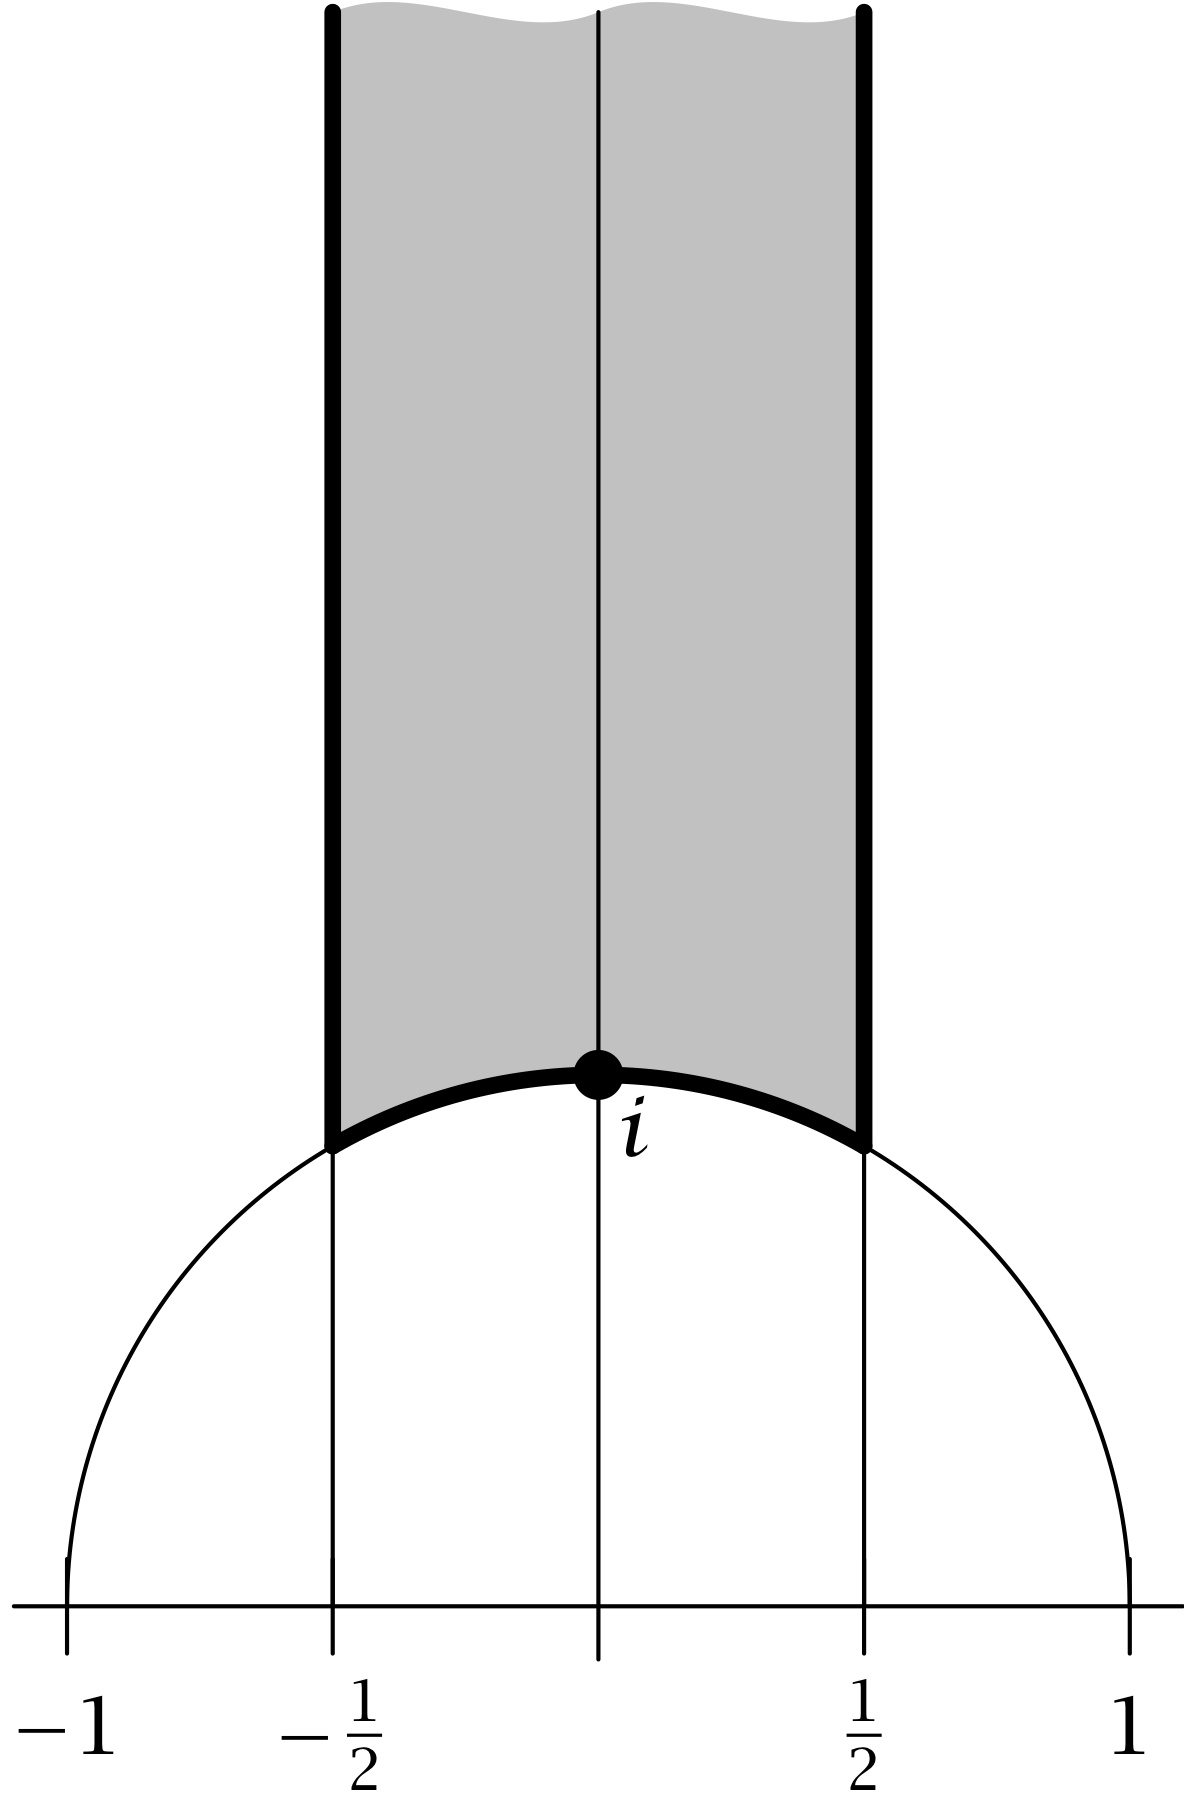
\includegraphics{PDF/SL2FundDom.jpg} $$
\subfigurename{a}. A fundamental domain $\overline{\fund_0}$.
\end{minipage}
%texpreamble
%(" \usepackage[LY1]{fontenc}
% \usepackage[expert, LY1, mylucidascale]{mylucidabr} % I adjusted the scaling
% \usepackage{amsmath}
% \everymath{\displaystyle}
% ");
%defaultpen(  fontcommand("\normalfont") + fontsize(10) ); 
%
%from graph access *;
%
%size(0,3inch);
%pair i = (0,1);
%real h = sqrt(3)/2;
%pair a = (-1/2, h);
%pair b = (1/2, h);
%real top = 3;
%filldraw( (1/2,h) .. i .. (-1/2,h)--(-1/2,top){ENE}..{ENE}(0,top){ENE}..{ENE}(1/2,top)--cycle , gray(0.8) , invisible  );
%draw( (-1/2,h)--(-1/2,top) , linewidth(2) );
%draw( (1/2,h)--(1/2,top) , linewidth(2) );
%draw( (-1/2,h) .. i .. (1/2,h) , linewidth(2) );
%draw( (-1,0){N}..(-1/2,h) .. i .. (1/2,h) .. {S}(1,0));
%draw( (-1/2,0) -- (-1/2,h) );
%draw( (1/2,0) -- (1/2,h) );
%dotfactor = 12;
%dot( i ); label( "$i$", (0,1), SE );
%real[] xticklist = {-1, -1/2, 1/2, 1};
%string labelfunc(real x){ 
%	if (x < -0.75){return "$-1$";} 
%	else if (x > 0.75) { return "$1$" ;}
%	else if (x < 0) { return "$\textstyle-\frac{1}{2}$" ;}
%	else if (x == 0) { return "$0$" ;}
%	else { return "$\textstyle\frac{1}{2}$" ;}
%	}
%xaxis(-1.1, 1.1, Ticks(xticklist, ticklabel=labelfunc) );
%yaxis(-0.1, top, true);
\qquad
\addtocounter{figure}{-1}
\renewcommand{\thefigure}{\oldthefigure(b)}
\refstepcounter{figure} \label{WeakFunDomSL2ZFig}
\begin{minipage}{\templength}
	$$ 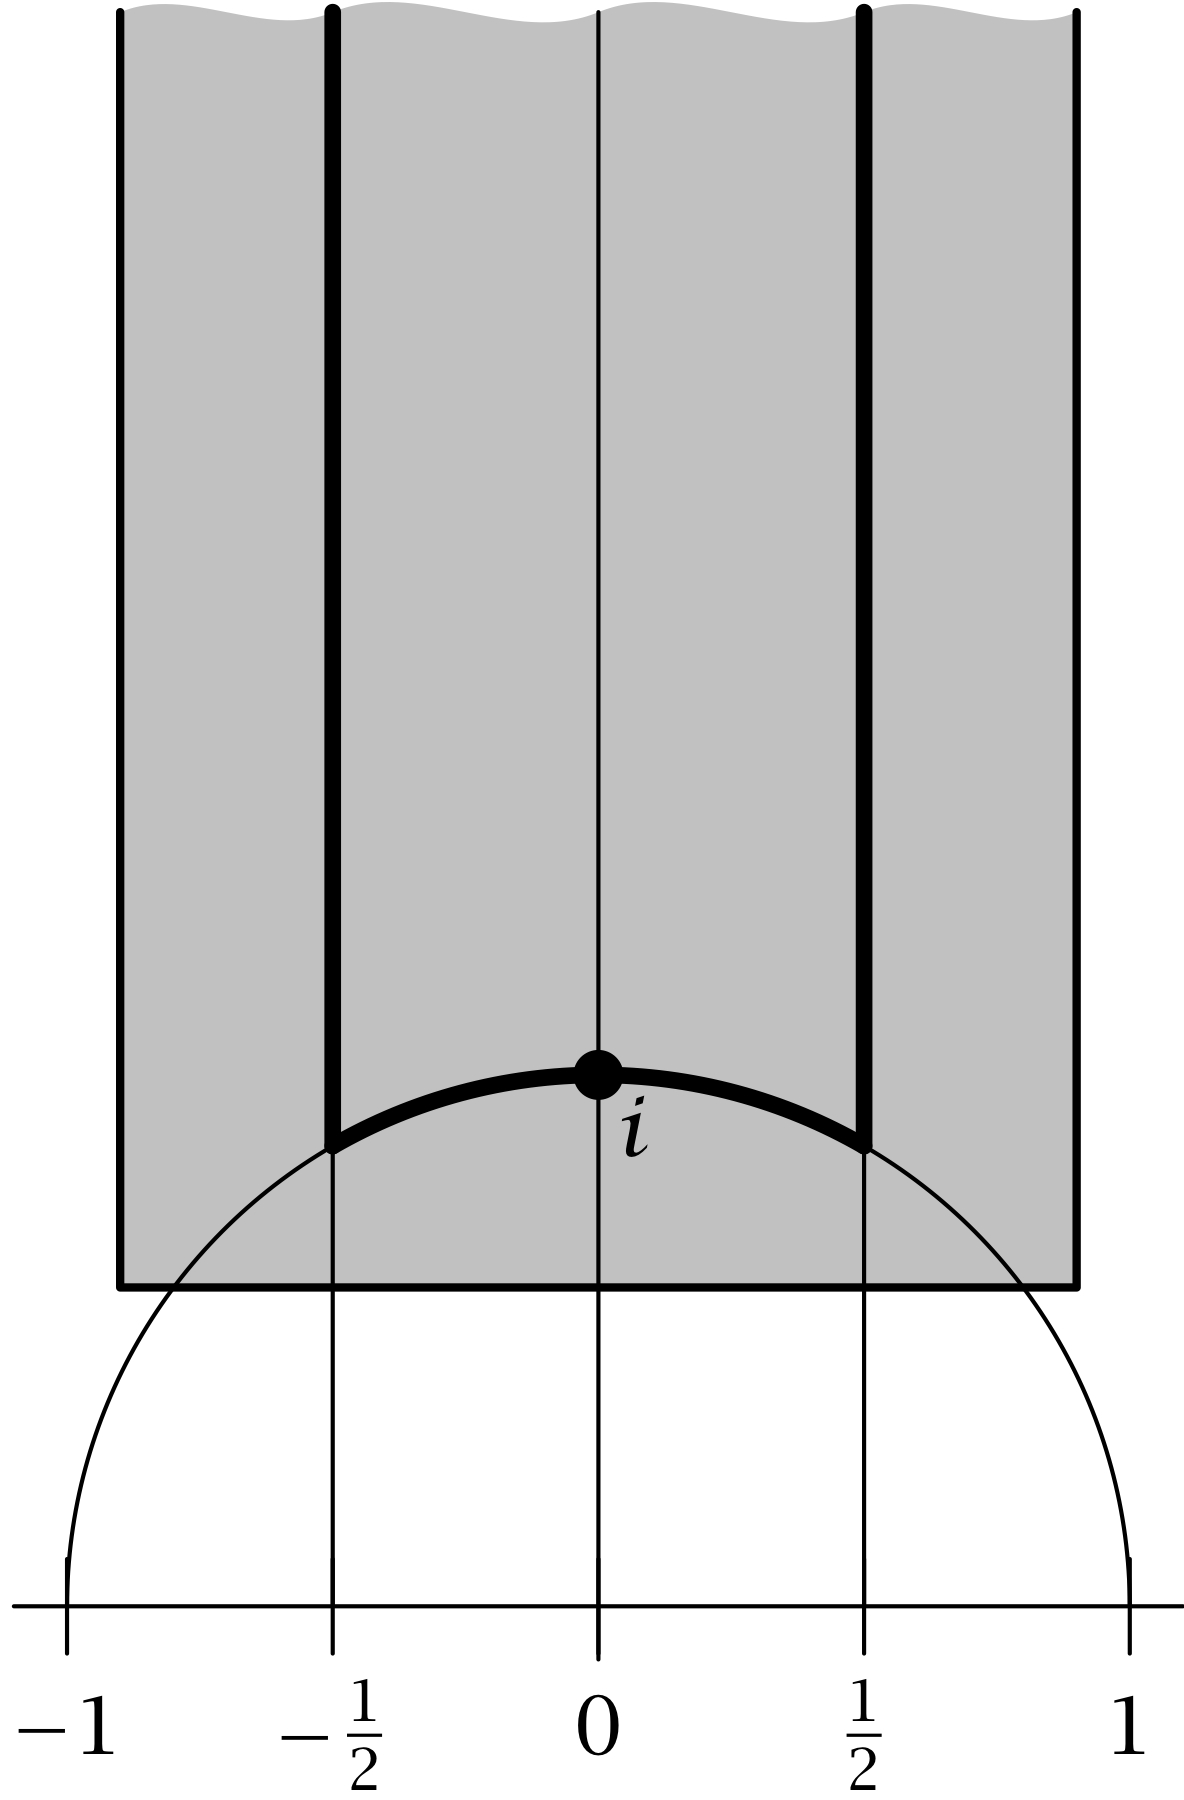
\includegraphics{PDF/SL2WeakFundDom.jpg} $$
\subfigurename{b}. A coarse fundamental domain~$\overline{\fund}$.
\end{minipage}
\end{figure}
%texpreamble
%(" \usepackage[LY1]{fontenc}
% \usepackage[expert, LY1, mylucidascale]{mylucidabr} % I adjusted the scaling
% \usepackage{amsmath}
% \everymath{\displaystyle}
% ");
%defaultpen(  fontcommand("\normalfont") + fontsize(10) ); 
%
%from graph access *;
%
%size(0,3inch);
%pair i = (0,1);
%real h = sqrt(3)/2;
%pair a = (-1/2, h);
%pair b = (1/2, h);
%real top = 3, x = 0.9, y = 0.6;
%filldraw( (x,y) -- (-x,y)--(-x,top){ENE}.. {ENE}(-1/2,top){ENE}..{ENE}(0,top){ENE}..{ENE}(1/2,top){ENE}..{ENE}(x,top)--cycle , gray(0.8) , invisible  );
%draw( (-x,top)--(-x,y)--(x,y)--(x,top), linewidth(1) );
%draw( (-1/2,h)--(-1/2,top) , linewidth(2) );
%draw( (1/2,h)--(1/2,top) , linewidth(2) );
%draw( (-1/2,h) .. i .. (1/2,h) , linewidth(2) );
%draw( (-1,0){N}..(-1/2,h) .. i .. (1/2,h) .. {S}(1,0));
%draw( (-1/2,0) -- (-1/2,h) );
%draw( (1/2,0) -- (1/2,h) );
%dotfactor = 12;
%dot( i ); label( "$i$", (0,1), SE );
%real[] xticklist = {-1, -1/2, 0, 1/2, 1};
%string labelfunc(real x){ 
%	if (x < -0.75){return "$-1$";} 
%	else if (x > 0.75) { return "$1$" ;}
%	else if (x < 0) { return "$\textstyle-\frac{1}{2}$" ;}
%	else if (x == 0) { return "$0$" ;}
%	else { return "$\textstyle\frac{1}{2}$" ;}
%	}
%xaxis(-1.1, 1.1, Ticks(xticklist, ticklabel=labelfunc) );
%yaxis(-0.1, top, true);

Unfortunately, the shape of~$\overline{\fund_0}$ is not entirely trivial, because the bottom edge is curved. Furthermore, the shape of a fundamental domain gets much more complicated when $G$ is larger than just $\SL(2,\real)$. Therefore, we will content ourselves with finding a set that is easier to describe, and is close to being a fundamental domain. 

\begin{eg}
To construct a region that is simpler than~$\overline{\fund_0}$, we can replace the curved edge with an edge that is straight. Also, because we do not need to find precisely a fundamental domain, we can be a bit sloppy about exactly where to place the edges, so we can enlarge the region slightly by moving the edges out a bit. The result is depicted in 
\cref{WeakFunDomSL2ZFig}. %on page~\pageref{WeakFunDomSL2ZFig}.
This new region~$\overline{\fund}$ is slightly larger than a fundamental domain, but it is within bounded distance of a fundamental domain,  and it suffices for many purposes. In particular, it is a coarse fundamental domain, in the sense of \cref{CoarseFundDomDefn} \csee{FIsWeakFundDom}.

An important virtue of this particular coarse fundamental domain is that it can be specified quite easily:
	$$ \overline{\fund} = \bigset{x + y i }{ \begin{matrix} c_1 \le x \le c_2, \\ y \ge c_3 \end{matrix} } $$
for appropriate $c_1, c_2, c_3 \in \real$.
\end{eg}

By using the Iwasawa decomposition $G = N A \, K$ \csee{{PermuteIwasawaSLnR}}, we can give a fairly simple description of the corresponding coarse fundamental domain~$\fund$ in $\SL(2,\real)$:

\begin{eg}  \label{SiegelSL2ZinSL2R}
Let
\noprelistbreak
	\begin{itemize}
	\item
	$\fund = \{\, g \in G \mid g(i) \in \overline{\fund} \,\}$, 
	\item $N_{c_1,c_2} = \bigset{
	\begin{bmatrix} 1 & t \\ 0 & 1 \end{bmatrix}
	}{
	c_1 \le t \le c_2}$, 
	\item $A_{c_3} = \bigset{
	\begin{bmatrix} e^t \\ &e^{-t} \end{bmatrix}
	}{
	e^{2t} \ge c_3}$,
	and
	\item $K = \SO(2)$.
	\end{itemize}
Then \csee{FIsSiegelSet}
	$$\fund = N_{c_1,c_2} A_{c_3} K  .$$
\end{eg}

Any set of the form $N_{c_1,c_2} A_{c_3} K$ is called a ``Siegel set\zz,''  so we can summarize this discussion by saying that Siegel sets provide good examples of coarse fundamental domains for $\SL(2,\integer)$ in $\SL(2,\real)$. 
%As a matter of notation, we mention that the gothic letter~$\Siegel$ is usually used to denote a Siegel set.

To construct a coarse fundamental domain for $\SL(n,\integer)$ (with $n > 2$), we generalize the notion of Siegel set to $\SL(n,\real)$.


\begin{defn}[(Siegel sets for $\SL(n,\integer)$)] \label{SiegelSLnZDefn}
Let $G = \SL(n,\real)$, and consider the Iwasawa decomposition $G = NAK$ \csee{PermuteIwasawaSLnR}.
To generalize \cref{SiegelSL2ZinSL2R}, we construct a ``Siegel set'' $\Siegel$ by choosing appropriate subsets $\overline{N}$ of~$N$ and $\overline{A}$ of~$A$, and letting $\Siegel = \overline{N} \, \overline{A} \, K$. 

\begin{itemize}
\item The set $\overline{N}$ can be any (nonempty) compact subset of~$N$. For example, we could let 
	$$\overline{N} = N_{c_1,c_2} = \{\, u \in N \mid \text{$c_1 \le u_{i,j} \le c_2$ for $i < j$} \,\} .$$
\item Note that the set $A_{c_3}$ of \cref{SiegelSL2ZinSL2R} has the following alternate description:
	$$ A_{c_3} = \{\, a \in A \mid a_{1,1} \ge c_3 \, a_{2,2} \,\}. $$
%since $e^t/e^{-t} = e^{2t}$. 
Therefore, we can generalize to $\SL(n,\real)$ by defining
	$$ A_c = \{\, a \in A \mid \text{$a_{i,i}   \ge c \, a_{i+i,i+1}$ for $i = 1,\ldots,n-1$} \,\} .$$
\end{itemize}
Thus, for $c_1,c_2 \in \real$ and $c_3 \in \real^+$, we have a Siegel set%
\nindex{$\Siegel_{c_1,c_2,c_3} = N_{c_1,c_2} A_{c_3} K$ is a Siegel set for $\SL(n,\integer)$}% no page break here !!!
	$$\Siegel_{c_1,c_2,c_3} = N_{c_1,c_2} A_{c_3} K .$$
\end{defn}

By calculating an appropriate multiple integral, it is not difficult to see that Siegel sets have finite measure:

\begin{prop}[\csee{SiegelSLnRFinMeasEx}] \label{SiegelSLnRFinMeas}
$\Siegel_{c_1,c_2,c_3}$ has finite measure\/ \textup(with respect to the Haar measure on\/ $\SL(n,\real)$\textup).
\end{prop}


\begin{exercises}

\item \label{FundInX->FundInG}
Suppose $H$ is a closed subgroup of~$G$, and $\overline{\fund}$ is a strict fundamental domain for the action of~$\Gamma$ on~$G/H$. For every $x \in G/H$, show that
	$$ \fund = \{\, g \in G \mid gx \in \overline{\fund}\,\} $$
is a strict fundamental domain for~$\Gamma$ in~$G$.

\item \label{F1inFinF2}
Suppose $\fund_1$ and $\fund_2$ are coarse fundamental domains for~$\Gamma$ in~$G$. Show that if $\fund_1 \subseteq \fund \subseteq \fund_2$, then $\fund$ is also a coarse fundamental domain for~$\Gamma$ in~$G$.

\item \label{FinUnionFundDomsIsWeak}
Suppose 
	\begin{itemize}
	\item $\fund$ is a coarse fundamental domain for the action of~$\Gamma$ on~$X$, 
	and
	\item  $F$ is a nonempty, finite subset of~$\Gamma$.
	\end{itemize}
Show that $F \fund = \bigcup_{f \in F} f \fund$ is also a coarse fundamental domain.

\item \label{CoarseInX->CoarseInG}
Suppose $H$ is a closed subgroup of~$G$, and $\overline{\fund}$ is a coarse fundamental domain for the action of~$\Gamma$ on~$G/H$. For every $x \in G/H$, show that
	$$ \fund = \{\, g \in G \mid gx \in \overline{\fund}\,\} $$
is a coarse fundamental domain for~$\Gamma$ in~$G$.

\item \label{FCoveredByF0}
In the notation of \cref{WeakAndFunDomSL2ZFig}, show that the coarse fundamental domain $\overline{\fund}$ is contained in the union of finitely many $\Gamma$-translates of the fundamental domain~$\overline{\fund_0}$.

\item \label{FIsWeakFundDom}
Show that the set $\overline{\fund}$ depicted in \cref{WeakFunDomSL2ZFig} is indeed a coarse fundamental domain for the action of~$\Gamma$ on~$\hyperbolic$. \hint{\Cref{FinUnionFundDomsIsWeak,FCoveredByF0}.  You may assume (without proof) that $\overline{\fund_0}$ is a fundamental domain.}

\item \label{WeakFundDomFinInd}
Suppose 
	\begin{itemize}
	\item $\fund$ is a coarse fundamental domain for $\Gamma$ in~$G$, 
	and
	\item  $F_1$ is a nonempty, finite subset of~$\Gamma$,
	and
	\item $\Gamma_1$ is a finite-index subgroup of~$\Gamma$. 
	\end{itemize}
Show:
	\begin{enumerate}
	\item that $F_1 \fund$ is also a coarse fundamental domain for $\Gamma$ in~$G$.
	\item \label{WeakFundDomFinInd-IsFund}
	If $\Gamma_1 F_1 \fund = G$, then $F_1 \fund$ is a  coarse fundamental domain for both $\Gamma$ and~$\Gamma_1$ in~$G$. 
	\end{enumerate}

\item Assume $\Gamma$ is infinite (or, equivalently, that $G$ is not compact), and $\Gamma_1$ is a finite-index, proper subgroup of~$\Gamma$. Show there exists a (strict) fundamental domain for $\Gamma_1$ in~$G$ that is \emph{not} contained in any coarse fundamental domain for $\Gamma$ in~$G$.
\hint{Construct a strict fundamental domain for $\Gamma_1$ that contains a strict fundamental domain~$\fund_0$ for~$\Gamma$, but is not covered by finitely many $\Gamma$-translates of $\fund_0$.}

\item \label{ConjFundDomsInGIsWeak}
Suppose 
	\begin{itemize}
	\item $\fund$ is a coarse fundamental domain for $\Gamma$ in~$G$, 
	and
	\item  $g \in \nzer_G(\Gamma)$.
	\end{itemize}
Show that  $\fund^g = g^{-1} \fund g$ is also a coarse fundamental domain.

\item \label{FIsSiegelSet}
Let $\fund$ be the coarse fundamental domain for $\SL(2,\integer)$ in $\SL(2,\real)$ that is  defined in \cref{SiegelSL2ZinSL2R}. Verify that $\fund = N_{c_1,c_2} A_{c_3} K$.
%\hint{We have
%	$K(i) = i$,
%	$A_{c_3} (i) = \{\, y i \mid y \ge c_3 \,\}$,
%	and $N_{c_1,c_2} \bigl( \{\, y i \mid y \ge c_3 \,\} \bigr) = \fund$.}

\item \label{Ac=aA+}
Let $G = \SL(n,\real)$. Given $c > 0$, show there exists $a \in A$, such that $A_c = a A^+$.

\item \label{HaarOnG=KAN}
\emph{This exercise provides a description of the Haar measure on~$G$.}

Let $dg$, $dk$, $da$, and $du$ be the Haar measures on the unimodular groups $G$, $K$, $A$, and~$N$, respectively, where $G = KAN$ is an Iwasawa decomposition. Also, for $a \in A$, let $\rho(a)$ be the modulus (or Jacobian) of the action of~$a$ on~$N$ by conjugation, so
	$$ \text{$\int_N f( a^{-1} u a) \, du = \int_N f(u) \, \rho(a) \, du$ for $f \in C_c(N)$} . $$
Show, for $f \in C_c(G)$, that
	\begin{align*}
	\int_G f \, dg 
	&=  \int_K \, \int_N \, \int_A \, f(kua) \, da \, du \, dk
	\\&= \int_K \, \int_A \, \int_N \, f(kau) \, \rho(a) \, du \, da \, dk
	. \end{align*}
\hint{Since $G$ is unimodular, $dg$ is invariant under left translation by elements of~$K$ and right translation by elements of~$AN$.}

\item \label{ModFuncANinSLnR}
Let $G = \SL(n,\real)$, choose $N$, $A$, and~$K$ as in \cref{SiegelSLnZDefn}, and 
define $\rho$ as in \cref{HaarOnG=KAN}. Show
	$$ \rho \left( \begin{Smallbmatrix} a_{1,1} \\&a_{2,2}
	\\ \BigSymbol{0}{0}{-5}&& \BigSymbol{0}{15}{15}\ddots \\&&& a_{n,n} \end{Smallbmatrix} \right) = \prod_{i<j} \frac{a_{j,j}}{a_{i,i}} .$$
%for all $a_{1,1},\ldots,a_{n,n} \in \real^+$.

\item \label{SiegelSLnRFinMeasEx}
Let $c_1,c_2,c_3 \in \real$, with $c_1 < c_2$ and $c_3 > 0$. Show that the Siegel set $\Siegel_{c_1,c_2,c_3}$ in $\SL(n,\real)$ has finite measure.
\hint{See \cref{HaarOnG=KAN,ModFuncANinSLnR} for a description of the Haar measure on $\SL(n,\real)$.}

\end{exercises}


\section{Constructive proof using Siegel sets} \label{SLNZISLATTSiegelPfSect}

In this section, we prove the following result:

\begin{thm} \label{SiegelFundDomSLnZ}
Let 
	\noprelistbreak
	\begin{itemize}
	\item $G = \SL(n,\real)$, 
	\item $\Gamma = \SL(n,\integer)$, 
	and 
	\item $\Siegel_{0,1,\frac{1}{2}} = N_{0,1} A_{1/2} K$ be the Siegel set defined in \cref{SiegelSLnZDefn}. 
	\end{itemize}
Then $G = \Gamma \, \Siegel_{0,1,\frac{1}{2}}$.
\end{thm}

This establishes \cref{SLNZISLATT}:

\begin{proof}[\bf Proof of \cref{SLNZISLATT}]
Combine the conclusion of \Cref{SiegelFundDomSLnZ} with \cref{SiegelSLnRFinMeas,Latt<>fund}.
\end{proof}

\begin{rems} \label{SiegelRemsLR} \ 
\noprelistbreak
	\begin{enumerate}
	\item \label{SiegelRemsLR-transpose}
	$\Gamma$ is written on the left in the conclusion of \cref{SiegelFundDomSLnZ}, because our definition of Siegel sets is motivated by a fundamental domain for the action of $\SL(2,\integer)$ on~$\hyperbolic^2$, and $\Gamma$~acts on the left there. However, taking the transpose of both sides of the conclusion of \cref{SiegelFundDomSLnZ} yields
		$ G = \Siegel_{0,1,\frac{1}{2}}^\transpose \Gamma$,
	where $\Siegel_{0,1,\frac{1}{2}}^\transpose = K A_{1/2} N_{c_1,c_2}^\transpose$. 
	Thus, $\Gamma$ can be written on the right, if the definition of Siegel set is modified appropriately.
	
	\item Our definition of Siegel sets uses the upper-triangular group~$N$, and \cref{SiegelFundDomSLnZ} puts $\Gamma$ on the left. Then \pref{SiegelRemsLR-transpose} uses the lower-triangular group~$N^\transpose$ (also called $N^-$), and puts $\Gamma$ on the right. Some authors reverse this, using $N^-$ when $\Gamma$ is on the left and using $N$ when the action on the right. However, to accomplish this, the inequality in the definition of~$A_c$ needs to be reversed. (See \cref{FundDomSL2ZinSL2RminEx} and the proof of \cref{SiegelFundDomSLnZ}.) 
	\end{enumerate}
\end{rems}

The following elementary observation is the crux of the proof of \cref{SiegelFundDomSLnZ}:

\begin{lem} \label{RedSLnZProjLem}
If $\Zlatt$ is any $\integer$-lattice in\/ $\real^n$, then there is an ordered basis $v_1,\ldots,v_n$ of\/~$\real^n$, such that
	\begin{enumerate}
	\item \label{RedSLnZProjLem-gen}
	$\{v_1,\ldots,v_n\}$ generates $\Zlatt$ as an abelian group,
	and
	\item \label{RedSLnZProjLem->1/2}
	$\| \proj_i^\perp v_{i+1} \| \ge \frac{1}{2} \| \proj_{i-1}^\perp v_{i} \|$ for\/ $1 \le i < n$, where\/ $\proj_i^\perp \colon \real^n \to V_i^\perp$ is the orthogonal projection onto the orthogonal complement of the subspace~$V_i$ spanned by\/ $\{v_1,v_2,\ldots,v_i\}$.
	\end{enumerate}
\end{lem}

\begin{proof}
Choose $v_1$ to be a nonzero vector of minimal length in~$\Zlatt$. Then define the remaining vectors $v_2,v_3,\ldots,v_n$ by induction, as follows:%
	\begin{itemize}
	\item[] Given $v_1,v_2,\ldots,v_i$, choose $v_{i+1} \in \Zlatt$ to make $\proj_i^\perp v_{i+1}$ as short as possible, subject to the constraint that $v_{i+1}$ is linearly independent from $\{v_1,v_2,\ldots,v_i\}$ \textup(so $\proj_i^\perp v_{i+1}$ is nonzero\/\textup). 
	\end{itemize}
We now verify \pref{RedSLnZProjLem-gen} and \pref{RedSLnZProjLem->1/2}.

\pref{RedSLnZProjLem-gen}
For each~$i$, let $\Zlatt_i$ be the abelian group generated by $v_1,v_2,\ldots,v_i$. If $\Zlatt_n \neq \Zlatt$, we may let $i$ be minimal with $\Zlatt_{i+1} \neq \Zlatt \cap V_{i+1}$. Then we must have $\proj_i^\perp \Zlatt_{i+1} \subsetneq \proj_i^\perp(\Zlatt \cap V_{i+1})$ \csee{RedSLnZProjX=YEx}, so there is some $v \in \Zlatt \cap V_{i+1}$ with $\proj_i^\perp v_{i+1} = k \cdot \proj_i^\perp v$ for some $k \ge 2$ \csee{RedSLnZProjCyclicEx}.  This contradicts the minimality of $\|\proj_i^\perp v_{i+1}\|$.

\pref{RedSLnZProjLem->1/2} 
For simplicity, assume $i = 1$ \csee{RedSLnZProj>1/2Ex}, and let $v_2^* = \proj_1^\perp v_2$, so $v_2 = v_2^* + \alpha v_1$, with $\alpha \in \real$. Obviously, there exists $k \in \integer$, such that $|\alpha - k| \le 1/2$. If 
		$ \| \proj_1^\perp v_2 \| <  \frac{1}{2} \| v_1 \| $,
then
	\begin{align*}
	 \|v_2 - k v_1\| 
	= \|v_2^* + (\alpha - k)v_1 \|
	&\le  \| v_2^*\| + |\alpha - k| \cdot \| v_1 \| 
	\\&< \frac{1}{2} \|v_1\| +  \frac{1}{2} \| v_1 \|
	= \|v_1 \| 
	. \end{align*}
This contradicts the minimality of ~$\|v_1\|$.
\end{proof}

\begin{proof}[\bf Proof of \cref{SiegelFundDomSLnZ}]
We wish to show $G = \Gamma \, \Siegel_{0,1,\frac{1}{2}} = \Gamma \, N_{0,1} \, A_{1/2} \, K$. However, since the proof uses an action of~$G$, and most readers prefer to have this action on the left, we will instead prove an analogous result with $\Gamma$ on the right: $G = \Siegel_{0,1,\frac{1}{2}}^{-} \Gamma$. 
%Roughly speaking, we take the inverse of both sides of the original equation. 
Namely, given $g \in G$, 
	$$ \text{we will show $g \in K \, A^-_{1/2} \, N_{0,1} \, \Gamma$,} $$
where $A^-_c = \{\, a^{-1} \mid a \in A_c \,\} = \{\, a \in A \mid \text{$a_{i,i} \le a_{i+1,i+1}/c$ for all~$i$} \,\}$.

For convenience, let $\Zlatt = g \integer^n$, and let $\{\varepsilon_1,\ldots,\varepsilon_n\}$ be the standard basis of~$\real^n$.  \Cref{RedSLnZProjLem} provides us with a sequence $v_1,\ldots,v_n$ of elements of~$\Zlatt$. From \fullref{RedSLnZProjLem}{gen}, we see that, after multiplying $g$ on the right by an element of~$\Gamma$, we may assume 
	$$ \text{$g \varepsilon_i = v_i$ for $i = 1,\ldots,n$} $$
\csee{eig=pmvi}. 

From the Iwasawa decomposition $G = KAN$ \csee{IwasawaDecompSLnR}, we may write
	$g = k a u$ with $k \in K$, $a \in A$, and $u \in N$.
For simplicity, let us assume $k$ is trivial \csee{SiegelSLnZ-knoteEx}, so
	$$ \text{$g = a u$ with $a \in A$ and $u \in N$.} $$
Since $g \in AN$, we know $g$ is upper triangular (and its diagonal entries are exactly the same as the diagonal entries of~$a$), so
	$$ \text{$\langle \varepsilon_1,\varepsilon_2,\ldots,\varepsilon_i \rangle
	= \langle g \varepsilon_1, g \varepsilon_2, \ldots, g\varepsilon_i \rangle 
	=  \langle v_1,v_2,\ldots,v_i \rangle$ for all~$i$} .$$
This implies that the diagonal entry $a_{i,i}$ of~$a$ is given by
	\begin{align*}
	a_{i,i}
	&=
	g_{i,i}
	=  \| \proj_{i-1}^\perp g \varepsilon_i \| 
	=  \| \proj_{i-1}^\perp v_i \| 
	\\& \le 2 \| \proj_i^\perp v_{i+1} \| 
	=  2\| \proj_i^\perp g \varepsilon_{i+1} \| 
	 = 2 g_{i+1,i+1} 
	 = 2 a_{i+1,i+1}
	 . \end{align*}
Therefore $a \in A_{1/2}^-$.

Also, there exists $ \gamma \in \Gamma \cap N$, such that
	$ u \in N_{0,1} \, \gamma$
\csee{N=NZN01}.
Therefore $g = a u \in  A_{1/2}^- \, N_{0,1} \, \gamma \subseteq  K \, A_{1/2}^- \, N_{0,1} \, \Gamma$, as desired.
\end{proof}


\begin{rem} \label{SiegelIsCoarseFundInSLnR}
	It can be shown that that the Siegel set $\Siegel_{0,1,\frac{1}{2}}$ is a coarse fundamental domain for $\SL(n,\integer)$ in $\SL(n,\real)$ \ccf{SiegelPropertySect}, but this fact is not needed in the proof that $\SL(n,\integer)$ is a lattice in $\SL(n,\real)$.
\end{rem}

\begin{exercises}

\item\label{FundDomSL2ZinSL2RminEx}
Let
	\begin{itemize}
	\item $N^-_{c_1,c_2} = \bigset{
	\begin{Smallbmatrix} 1 & 0 \\ t & 1 \end{Smallbmatrix}
	}{
	c_1 \le t \le c_2}$, 
	\smallskip % @@@
	\item $A^-_{c_3} = \bigset{
	\begin{Smallbmatrix} e^t\\ &e^{-t} \end{Smallbmatrix}
	}{
	e^{2t} \le c_3}$,
	\smallskip % @@@
	\item $K = \SO(2)$,
	and
	\item $\fund' = N^-_{c_1,c_2} A^-_{c_3} K $.
	\end{itemize}
Show that $\fund'$ is a coarse fundamental domain for $\SL(2,\integer)$ in $\SL(2,\real)$ if and only if the set $\fund = N_{c_1,c_2} A_{c_3} K$ of \cref{SiegelSL2ZinSL2R} is a coarse fundamental domain.
\hint{Conjugate by $\begin{Smallbmatrix} 0 & 1 \\ 1 & 0 \end{Smallbmatrix}$.}

\item \label{RedSLnZProjX=YEx}
In the notation of \cref{RedSLnZProjLem}, show that if $X$ and~$Y$ are two subgroups of $V_{i+1}$, such that 
	$$ \text{$X \subseteq Y$, 
	\ $X \cap V_i = Y \cap V_i$,
	\ and
	\ $\proj_i^\perp X = \proj_i^\perp Y$,} $$
then $X = Y$.

\item \label{RedSLnZProjCyclicEx}
In the notation of \cref{RedSLnZProjLem}, show that the group $\proj_i^\perp(\Zlatt \cap V_{i+1})$ is cyclic.
\hint{Since $\dim \proj_i^\perp V_{i+1} = 1$, it suffices to show $\proj_i^\perp(\Zlatt \cap V_{i+1})$ is discrete.}

\item \label{RedSLnZProj>1/2Ex}
Prove \fullcref{RedSLnZProjLem}{>1/2} without assuming $i = 1$.
\hint{Mod out $V_{i-1}$, which is in the kernel of both $\proj_{i-1}^\perp$ and $\proj_i^\perp$.}

\item 
For $g \in \GL(n,\real)$, show $g \in \GL(n,\integer)$ if and only if $g \integer^n \subseteq \integer^n$ and $g^{-1} \integer^n \subseteq \integer^n$.

\item \label{eig=pmvi}
For every $n$-element generating set $\{v_1,\ldots,v_n\}$ of the group~$\integer^n$, show there exists $\gamma \in \SL(n,\integer)$, such that $g \varepsilon_i = \pm v_i$ for every~$i$.
\hint{Show there exists $\gamma \in \GL(n,\integer)$, such that $g \varepsilon_i =  v_i$ for every~$i$.}

\item \label{SiegelSLnZ-knoteEx}
Complete the proof of \cref{SiegelFundDomSLnZ}  (without assuming the element~$k$ is trivial).
\hint{The group~$K$ acts by isometries on~$\real^n$, so replacing $\{v_1,\ldots,v_n\}$ with its image under an element of~$K$ does not affect the validity of \fullref{RedSLnZProjLem}{>1/2}.}

\item \label{N=NZN01}
For all $c \in \real$, show $N =  N_{c, c+1} N_{\integer}$.


\end{exercises}




\section{Elegant proof using nondivergence of unipotent orbits} \label{SLNZISLATTSlickSect}

We now present a very nice proof of \cref{SLNZISLATT} that relies on two key facts: the Moore Ergodicity Theorem \pref{MooreErgBasicThm}, and an important observation about orbits of unipotent elements (\cref{DaniMargulisUnipReturns}).
%that is often called the ``\term{Margulis Lemma}\zz.'' 
The statement of this observation will be more enlightening after some introductory remarks.

\begin{eg} \label{SplitDivergeSL2R}
Let $a = \begin{Smallbmatrix} 2& 0 \\ 0 & 1/2 \end{Smallbmatrix}$, or, more generally, let $a$ be any element of $\SL(2,\real)$ that is diagonalizable over~$\real$ (and is not~$\pm\Id$). Then $a$ has one eigenvalue that is greater than~$1$, and one eigenvalue that is less than~$1$ (in absolute value), so it is obvious that there exist linearly independent vectors $v_+$ and~$v_-$ in~$\real^2$, such that 
	$$ \text{$a^k v_+ \to 0$ \ and \ $a^{-k} v_- \to 0$ \  as $k \to +\infty$} . $$
By the Mahler Compactness Criterion \pref{MahlerCpct}, this implies that some of the orbits of~$a$ on $\SL(2,\real)/\SL(2,\integer)$ are ``divergent'' or ``go off to infinity'' or ``leave compact all sets\zz.'' That is, there exists $x \in \SL(2,\real)/\SL(2,\integer)$, such that, for every compact subset~$C$ of~$\SL(2,\real)/\SL(2,\integer)$,
	$$ \text{$\{\, k \in \integer \mid a^k x \in C \,\}$ is finite} $$
\csee{SplitDivergeSL2REx}. 
\end{eg}

In contrast, if $u = \begin{Smallbmatrix} 1 & 1 \\ 0 & 1 \end{Smallbmatrix}$, then it is clear that there does \emph{not} exist a nonzero vector $v \in \real^2$, such that $u^k v \to 0$ as $k \to \infty$. In fact, if $v$ is not fixed by~$u$ (i.e., if $uv \neq v$), then
	\begin{align} \label{unvtoinfty}
	\text{$\|u^k v \| \to \infty$ as $k \to \pm \infty$}
	\end{align}
\csee{UnipToInftyInR2}.
Therefore, it is not very difficult to show that \emph{none} of the orbits of~$u$ on $\SL(2,\real)/\SL(2,\integer)$ go off to infinity:

\begin{prop} \label{MargulisRecurSL2R}
If $u$ is any unipotent element of\/ $\SL(2,\real)$, then, for all $x \in \SL(2,\real)/\SL(2,\integer)$, there is a compact subset~$C$ of\/ $\SL(2,\real)/\SL(2,\integer)$, such that
	$$ \text{$\{\, k \in \integer^+ \mid u^k x \in C \,\}$ is infinite} .$$
\end{prop}

\begin{proof}
We may assume $u$ is nontrivial. Then, by passing to a conjugate (and perhaps taking the inverse), we may assume $u = \left[\begin{smallmatrix} 1 & 1 \\ 0 & 1 \end{smallmatrix} \right]$.

Choose a small neighborhood~$\open\mk$ of~$0$ in~$\real^2$ so that, for all $g \in \SL(2,\real)$, there do not exist two linearly independent vectors in $\open\mk \cap g \integer^2$ \csee{2SmallNotIndep}. Since $x \integer^2$ is discrete, we may assume $\open\mk$ is small enough that 
	\begin{align} \label{OpenNotXZ2}
	\open\mk \cap x \integer^2 = \{0\}
	. \end{align}
Since $\open\mk$ is open and $0$ is a fixed point of~$u$ (and the action of~$u^{-1}$ is continuous), there exists $r > 0$, such that
	\begin{align} \label{uBrInOpen}
	 B_r(0) \cup u^{-1} B_r(0) \subseteq \open 
	 , \end{align}
where $B_r(0)$ is the open ball of radius~$r$ around~$0$.
Let 
	$$ C = \bigset{ c \in \SL(2,\real)/\SL(2,\integer) }{ c \integer^2 \cap B_r(0) = \{0\} } .$$
The Mahler Compactness Criterion \pref{MahlerCpct} tells us that $C$ is compact.

Given $N \in \integer^+$, it suffices to show there exists $k \ge 0$, such that $u^{N+k} x \in C$. That is,
	$$\text{we wish to show there exists $k \ge 0$, such that $u^{N+k} x \integer^2 \cap B_r(0) = \{0\}$} . $$
Let $v$ be a nonzero vector of smallest length in $u^N x \integer^2$. We may assume $\|v\| < r$ (for otherwise we may let $k = 0$). Hence, \pref{OpenNotXZ2} implies that $v$ is not fixed by~$u$. Then, from \pref{unvtoinfty}, we know there is some $k > 0$, such that $\|u^k v\| \ge r$, and we may assume $k$ is minimal with this property. Therefore $\|u^{k-1} v \|< r$, so $u^{k-1} v \in B_r(0) \subseteq \open$\, by \pref{uBrInOpen}.

From the choice of~$\open$, we know that $\open \cap u^{N+k-1} x \integer$ does not contain any vector that is linearly independent from~$u^{k-1} v$. Therefore $u^{N+k} x \integer^2$ does not contain any nonzero vectors of length less than~$r$ \csee{MargulisSL2RNotLessR}, as desired.
\end{proof}

This result has a natural generalization to $\SL(n,\real)$ (but the proof is more difficult; see \cref{PfUnipOrbitsReturnSect}):

\begin{thm}[(Margulis)] 
\label{MargulisUnipReturns}
Suppose
\noprelistbreak
	\begin{itemize}
	\item $u$ is a unipotent element of\/ $\SL(n,\real)$,
	and
	\item $x \in \SL(n,\real)/\SL(n,\integer)$.
	\end{itemize}
Then there exists a compact subset~$C$ of\/ $\SL(n,\real)/\SL(n,\integer)$, such that
	$$ \text{$\{\, k \in \integer^+ \mid u^k x \in C \,\}$ is infinite} .$$
\end{thm}

In other words, every unipotent orbit visits some compact set infinitely many times. In fact, it can be shown that the orbit visits the compact set quite often --- it spends a nonzero fraction of its life in the set:

\begin{thm}[(Dani-Margulis)]
 \label{DaniMargulisUnipReturns}
Suppose
	\begin{itemize}
	\item $u$ is a unipotent element of\/ $\SL(n,\real)$,
	and
	\item $x \in \SL(n,\real)/\SL(n,\integer)$.
	\end{itemize}
Then there exists a compact subset~$C$ of\/ $\SL(n,\real)/\SL(n,\integer)$, such that
	$$ \liminf_{m \to \infty} \frac{\# \bigset{ k \in \{1,2,\ldots,m\} }{ u^k x \in C} }{m} > 0 .$$
\end{thm}

Before saying anything about the proof of this important fact, let us see how it implies the main result of this chapter:

\begin{proof}[\bf Proof of \cref{SLNZISLATT}]
Let 
	\begin{itemize}
	\item $X = \SL(n,\real)/\SL(n,\integer)$,
	and
	\item $\mu$ be an $\SL(n,\real)$-invariant measure on~$X$ \csee{HaarOnHomog}.
	\end{itemize}
We wish to show $\mu(X) < \infty$.

Fix a nontrivial unipotent element~$u$ of $\SL(n,\real)$. For each $x \in X$ and compact $C \subseteq X$, let
	\begin{align*}
	 \rho_C( x ) 
	 &= \liminf_{m \to \infty} \frac{ \# \bigset{ k \in \{1,2,\ldots,m\} }{ u^k x \in C }  } {m} 
	 . \end{align*}
Since $X$ can be covered by countably many compact sets, \cref{DaniMargulisUnipReturns} implies there is a compact set~$C$, such that
	\begin{align} \label{rhoC>0}
	 \text{$\rho_C > 0$ on a set of positive measure} 
	 \end{align}
\csee{rhoC>0Ex}. 
Letting $\chi_C$ be the characteristic function of~$C$, we have
	\begin{align*}
	\int_X \rho_C  \, d\mu
	&= \int_X \liminf_{m \to \infty} \frac{ \# \! \bigset{ k \in \{1,2,\ldots,m\} }{ u^k x \in C }  } {m} \, d\mu(x)
	\\&\le  \liminf_{m \to \infty} \int_X  \! \frac{ \# \! \bigset{ k \in \{1,2,\ldots,m\} }{ u^k x \in C }  } {m} \, d\mu(x)
	 \vbox to 0pt{\vss\vskip-5pt\hbox{\hskip0.07in$\begin{pmatrix} \text{Fatou's} \\ \text{Lemma} \\ \text{\pref{FatousLemma}} \end{pmatrix}$}\vss} % is the spacing good? @@@
	\\&=  \liminf_{m \to \infty} \frac{1}{m} \int_X  \bigl( \chi_{u^{-1}C} + \chi_{u^{-2}C} + \cdots  + \chi_{u^{-m}C} \bigr) \, d\mu
	\\&= \liminf_{m \to \infty}  \frac{1}{m} \left( \int_X \chi_{u^{-1}C}  \, d\mu + \int_X \chi_{u^{-2}C}  \, d\mu + \cdots  
		+ \int_X \chi_{u^{-m}C}   \, d\mu \right)
	\\&= \liminf_{m \to \infty} \frac{1}{m} \Bigl( \mu( u^{-1} C ) +  \mu( u^{-2} C ) + \cdots  
		+  \mu( u^{-m} C ) \Bigr)
	\\&= \liminf_{m \to \infty} \frac{1}{m} \Bigl( \mu(C) +  \mu(C)  + \cdots  +  \mu(C) \Bigr)
	\\&= \mu(C)
	\\&< \infty
	, \end{align*}
so $\rho_C \in \LL1(X, \mu)$.

It is easy to see that $\rho_C$ is $u$-invariant \csee{rhoCinvtEx}, so the Moore Ergodicity Theorem \pref{MooreErgBasicThm} implies that $\rho_C$ is constant (a.e.).
Also, from \pref{rhoC>0}, we know that the constant is not~$0$. Therefore, we have a nonzero constant function that is in $\LL1(X,\mu)$, which tells us that $\mu(X)$ is finite.
\end{proof}

Now, to begin our discussion of the proof of \cref{DaniMargulisUnipReturns}, we introduce a bit of terminology and notation, and make some simple observations. First of all, let us restate the result by using the Mahler Compactness Criterion \pref{MahlerCpct}, and also replace the discrete times $\{1,2,3,\ldots,m\}$ with a continuous interval $[0,T]$. \Cref{SpendTimeCpctMahlerEx} shows that this new version implies the original.

\begin{defn} \label{UnimodLattDefn}
For any $\integer$-lattice~$\Zlatt$ in~$\real^n$, there is some $g \in \GL(n,\real)$, such that $\Zlatt = g \integer^n$. We say $\Zlatt$ is \defit[Z-lattice@$\integer$-lattice!unimodular]{unimodular} if $\det g = \pm 1$.
\end{defn}

\begin{thm}[(restatement of \cref{DaniMargulisUnipReturns})] \label{SpendTimeCpctMahler}
Suppose
\noprelistbreak
	\begin{itemize}
	\item $\{u^t\}$ is a one-parameter unipotent subgroup of\/ $\SL(n,\real)$,
	\item $\Zlatt$ is a unimodular $\integer$-lattice in\/~$\real^n$,
	and
	\item \nindex{$\leb$ = Lebesgue measure on~$\real$}$\leb$ is the usual Lebesgue measure\/ \textup(i.e., length\/\textup) on\/~$\real$.
	\end{itemize}
Then there exists a neighborhood~$\open$ of\/~$0$ in\/~$\real^n$, such that
	$$ \liminf_{T \to \infty} \frac{\leb \Bigl( \bigset{ t \in [0,T] }{ u^t \Zlatt \cap \open = \{0\} } \Bigr)}{T} > 0 .$$
\end{thm}



\begin{notation} \label{PrimVecDefn}
Suppose $W$ is a discrete subgroup of~$\real^n$. 
\noprelistbreak
	\begin{itemize}
	\item A vector $w \in W$ is \defit[primitive vector]{primitive} in~$W$ if $\lambda w \notin W$, for $0 < \lambda < 1$.
	\item Let \nindex{$\prims{W}$ = $\{\text{primitive vectors in discrete subgroup~$W$ of $\real^n$}\}$}$\prims{W}$ 
	be the set of primitive vectors in~$W$.
	\item Let 
	\nindex{$\primplus{W}$ = set of representatives of $\prims{W}/\{\pm1\}$}$\primplus{W} \subseteq \prims{W}$ be a set of representatives that contains either~$w$ or~$-w$, but not both, for every $w \in \prims{W}$.
	(Note that $\prims{W} = -\prims{W}$; see \cref{PrimVecIffEx}.)
	\end{itemize}
\end{notation}

For simplicity, let us assume now that $n = 2$ (see \cref{PfUnipOrbitsReturnSect} for a discussion of the general case).

\begin{lem} \label{SmallPrimsInUnimodLatt} \ 
\noprelistbreak
	\begin{enumerate}
	\item \label{SmallPrimsInUnimodLatt-1}
There is a neighborhood~$\open_1$ of\/~$0$ in\/~$\real^2$, such that if $W$ is any unimodular $\integer$-lattice in\/~$\real^2$, then\/ $\# \!\left(\primplus{W} \cap \open_1\right) \le 1$.
	\item \label{SmallPrimsInUnimodLatt-compare}
Given any neighborhood~$\open_1$ of\/~$0$ in\/~$\real^2$, and any $\epsilon > 0$, there exists a neighborhood~$\open_2$ of\/~$0$ in\/~$\real^2$, such that if $x \in \real^2$, and\/ $[a,b]$ is an interval in\/~$\real$, such that there exists $t \in [a,b]$ with $u^t x \notin \open_1$, then
		$$ \leb \left( \bigset{ t \in [a,b] }{ u^t x \in \open_2 } \right) 
		\le \epsilon \, \leb \left( \bigset{ t \in [a,b] }{ u^t  x \in \open_1 } \right) . $$
	\end{enumerate}
\end{lem}

\begin{figure}[ht]
\begin{center}
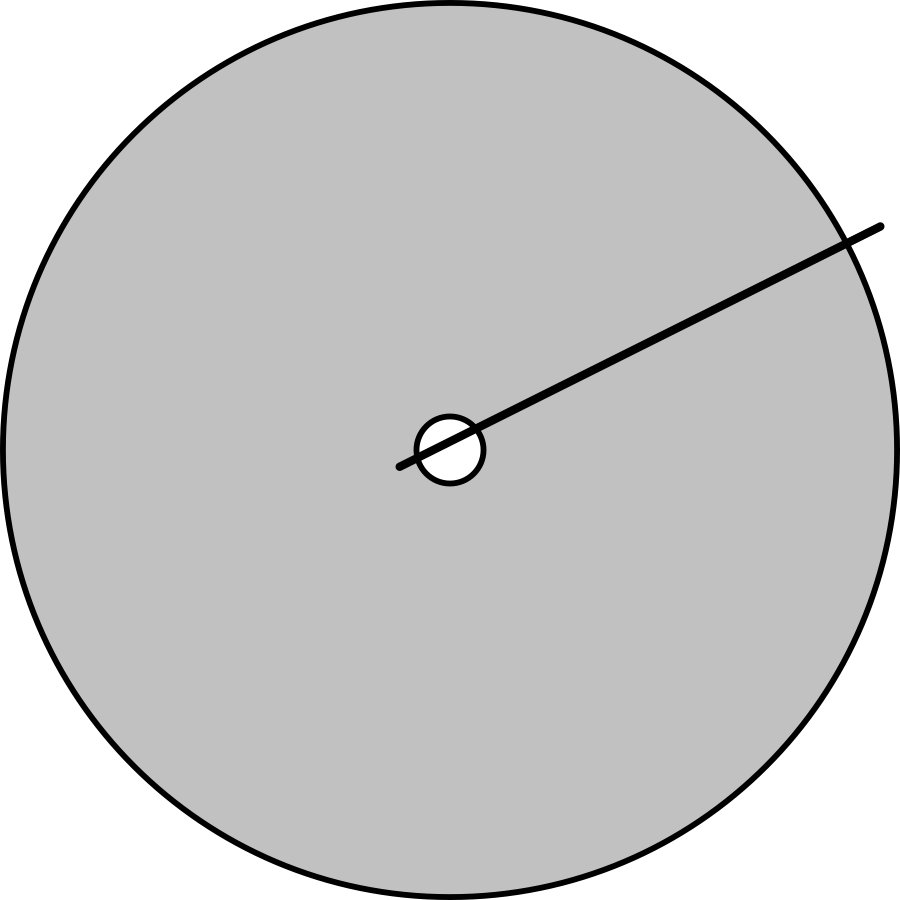
\includegraphics{PDF/line-seg-in-small-disk.jpg}
\end{center}
\caption{Part~\pref{SmallPrimsInUnimodLatt-compare} of \cref{SmallPrimsInUnimodLatt}: Any line segment that reaches the boundary of the large disk has only a small fraction of its length inside the tiny disk.}
\label{LineSegSmallTimeInSmallDisk}
\end{figure}
%texpreamble
%(" \usepackage[T1]{fontenc}
% \usepackage[expert, T1, nofontinfo, mylucidascale]{mylucidabr}
% \usepackage{amsmath}
% ");
%defaultpen(  fontcommand("\normalfont") + fontsize(10) ); 
%
%from graph access *;
%
%size(0,1.5inch);
%
%real R = 2, r = 0.15;
%
%//xaxis(-R-r,R+r);
%//yaxis(-R-r,R+r);
%
%fill( (R,0)..(0,R)..(-R,0)..(0,-R)..cycle, gray(0.8) );
%draw( (R,0)..(0,R)..(-R,0)..(0,-R)..cycle, linewidth(0.7) );
%fill( (r,0)..(0,r)..(-r,0)..(0,-r)..cycle, white );
%draw( (r,0)..(0,r)..(-r,0)..(0,-r)..cycle, linewidth(0.7) );
%
%draw( (-3/2*r,-r/2)--(R-r/2, 0.5*R ) , linewidth(1) );

\begin{proof} 
\pref{SmallPrimsInUnimodLatt-1}~A unimodular $\integer$-lattice in~$\real^2$ cannot contain two linearly independent vectors of norm less than~$1$ \csee{UnimodNot2Short}.

\pref{SmallPrimsInUnimodLatt-compare} Note that $u^t x$ moves at constant velocity along a straight line \csee{UnipOrbIsLine}. So we simply wish to choose~$\open_2$ small enough that every line segment that reaches the boundary of~$\open_1$ has only a small fraction of its length inside~$\open_2$ \ccf{LineSegSmallTimeInSmallDisk}.

By making $\open_1$ smaller, there is no harm in assuming it is a disk centered at~$0$. Let $R$ be the radius of~$\open_1$, and let $\open_2$ be a disk of radius~$r$ centered at~$0$, with $r$ small enough that
	$$ \frac{2r}{R - r} < \epsilon .$$
Then, for any line segment~$L$ that reaches both $\open_2$ and the boundary of~$\open_1$, we have:
	\begin{itemize}
	\item the length of $L \cap \open_2$ is $\le$ the diameter $2r$ of $\open_2$,
	and
	\item the length of $L \cap \open_1$ is $\ge$ the distance $R - r$ from $\bdry \open_1$ to $\bdry \open_2$.
	\end{itemize}
Therefore, the segment of~$L$ that is in~$\open_2$ has length less than $\epsilon$ times the length of the segment that is~$\open_1$  \ccf{LineSegSmallTimeInSmallDisk}.
\end{proof}

\begin{proof}[\mathversion{bold}\bf Proof of \cref{SpendTimeCpctMahler} when $n = 2$]
Let $\open_1$ and $\open_2$ be as described in \cref{SmallPrimsInUnimodLatt}, with $\epsilon = 1/2$.
We may assume $\open_1$ and~$\open_2$ are convex, that they are small enough that they contain no nonzero elements of~$\Zlatt$, and that $\open_2 \subseteq \open_1$.

Fix $T \in \real^+$. For each $x \in \primplus{\Zlatt}$, and $k = 1,2$, let 
	$$ I^k_x = \{\, t \in [0,T] \mid x u^t  \in \open_k \,\} .$$
Since $\open_k$ is convex, and $u^t x$ traces out a line \csee{UnipOrbIsLine}, we know that $I^k_x$ is an interval (possibly empty). Note that:
	\begin{enumerate}
	\item  from \fullcref{SmallPrimsInUnimodLatt}{compare} (and the fact that $\epsilon = 1/2$), we see that 
	$ \leb( I^2_x ) \le \frac{1}{2} \leb( I^1_x )  $,
	and
	\item  from  \fullcref{SmallPrimsInUnimodLatt}{1}, we see that $I^1_{x_1}$ is disjoint from $I^1_{x_2}$ whenever $x_1 \neq x_2$.
	\end{enumerate}
Therefore
	\begin{align*}
	 \leb \bigl( \{\, t \in [0,T] \mid u^t \Zlatt  \cap \open_2 & \neq \{0\} \bigr) 
	= \sum_{x \in \primplus{\Zlatt}} \leb( I^2_x ) 
	\le \sum_{x \in \primplus{\Zlatt}} \frac{\leb( I^1_x )}{2}
	\\&= \frac{1}{2} \leb \left(  \bigcup_{x \in \primplus{\Zlatt}} I^1_x  \right)
	\le \frac{1}{2} \leb \bigl(  [0,T] \bigr)
	=  \frac{T}{2} 
	. \end{align*}
So, passing to the complement, we have
	\begin{align*}
	\leb \bigl( \{\, t \in [0,T] \mid u^t \Zlatt \cap \open_2 = \{0\} \bigr) 
	\ge \frac{T}{2} 
	. & \qedhere \end{align*}
\end{proof}

Unfortunately, \cref{SpendTimeCpctMahler} is not nearly as easy to prove when $n > 2$, because two basic complications arise.
	\begin{enumerate}
	\item The first difficulty is that the $u^t$-orbit of a vector is usually not a straight line (contrary to \cref{UnipOrbIsLine} for $n = 2$). However, the coordinates of $u^t x$ are always polynomials of bounded degree \csee{UnipOrbsArePoly}, so, for any fixed vector~$x$, 
	$$ \text{the function $\| u^t x \|^2$ is a polynomial in~$t$} $$
and the degree of this polynomial is bounded (independent of~$x$).
Therefore, it is easy to prove that the appropriate analogue of \fullcref{SmallPrimsInUnimodLatt}{compare} holds even if $n > 2$ \csee{PolySpendsLittleTimeSmall}, so the nonlinearity is not a major problem.

	\item A much more serious difficulty is the failure of \fullref{SmallPrimsInUnimodLatt}{1}: if $n > 2$, then a unimodular lattice in~$\real^n$ may have two  linearly independent primitive vectors that are very small \csee{UnimodLattCanHaveLotsSmallVectors}. This means that the sets $I^2_x$ in the above proof may not be disjoint, which is a major problem. It is solved by looking at not only single vectors, but at larger sets of linearly independent vectors. More precisely, we look at the subgroups generated by sets of small vectors in~$u^t \Zlatt$. These subgroups can intersect in rather complicated ways, and sorting this out requires a study of chains of these subgroups (ordered by inclusion) and a rather delicate proof by induction. 
Although the proof is completely elementary, using only some observations about polynomial functions, it is very clever and intricate. The main idea is presented in \cref{PfUnipOrbitsReturnSect}.
	\end{enumerate}


\begin{exercises}


\item \label{SplitDivergeSL2REx}
Suppose $a \in \SL(2,\real)$, and there exist linearly independent vectors $v_+$ and~$v_-$ in~$\real^2$, such that 
	$$ \text{$a^n v_+ \to 0$ as $n \to +\infty$ \ and \ $a^n v_- \to 0$ as $n \to -\infty$} . $$
Show $\exists$~$x \in \SL(2,\real)/\SL(2,\integer)$, such that $\{\, n \in \integer \mid a^n x \in C \,\}$ is finite, for every compact subset~$C$ of~$\SL(2,\real)/\SL(2,\integer)$.
\hint{There exists $g \in \SL(2,\real)$ that takes the two standard basis vectors of~$\real^2$ to vectors that are scalar multiples of $v_+$ and~$v_-$.}

\item \label{UnipToInftyInR2}
Let $u = \left[\begin{smallmatrix} 1 & 1 \\ 0 & 1 \end{smallmatrix}\right]$. For every $v \in \real^2$, show that either 
	\begin{itemize}
	\item $u^n v = v$ for all $n \in \integer$,
	or
	\item $\|u^n v\| \to \infty$ as $n \to \infty$.
	\end{itemize}

\item
Generalize the preceding exercise to $\SL(n,\real)$:
\par
Let $u$ be any unipotent element of $\SL(n,\real)$. For every $v \in \real^n$, show that either 
	\begin{itemize}
	\item $u^n v = v$ for all $n \in \integer$,
	or
	\item $\|u^n v\| \to \infty$ as $n \to \infty$.
	\end{itemize}
\hint{Each coordinate of $u^n v$ is a polynomial function of~$n$, and non-constant polynomials cannot be bounded.}

\item \label{2SmallNotIndep}
Suppose $v_1$ and~$v_2$ are linearly independent vectors in~$\integer^2$, and we have $g \in \SL(2,\real)$. Show that if $\|gv_1\| < 1$, then $\|g v_2\| > 1$.
\hint{Since $g \in \SL(2,\real)$, the area of the parallelogram spanned by the vectors $g v_1$ and~$g v_2$ is the same as the area of the parallelogram spanned by $v_1$ and~$v_2$, which is an integer.}

\item \label{MargulisSL2RNotLessR}
Near the end of the proof of \cref{MargulisRecurSL2R}, verify the assertion that $u^{n+N} x \integer^2$ does not contain any nonzero vectors of length less than~$r$.
\hint{If $\|w\| < r$, then $u^{n-1}v$ and $u^{-1} w$ are linearly independent vectors in $\open \cap u^{n+N-1} x \integer$.}

\item \label{rhoC>0Ex}
Prove \pref{rhoC>0}.
\hint{$X$ cannot be the union of countably many sets of measure~$0$.}

\item \label{rhoCinvtEx}
In the proof of \cref{SLNZISLATT}, verify (directly from the definition) that $\rho_C$ is $u$-invariant.

\item \label{UnimodLattDefnWellDef}
Show \cref{UnimodLattDefn} is well-defined. More precisely, given any $g_1 , g_2 \in \GL(n,\real)$, such that $g_1 \integer^n = g_2 \integer^n$, show 
	$$ \det g_1 \in \{ \pm1\}  \iff \det g_2 \in \{ \pm 1\} .$$

\item \label{DiscToContInCpct}
Assume 
	\begin{itemize}
	\item $u^t$ is a one-parameter unipotent subgroup of~$G$, 
	\item $x \in G/\Gamma$,
	and
	\item $C^*$ is a compact subset of $G/\Gamma$.
	\end{itemize}
Show that if 
	$$ \liminf_{T \to \infty} \frac{\leb \Bigl( \bigset{ t \in [0,T] }{  u^t x \in C^* } \Bigr)}{T} > 0 , $$
then there is a compact subset~$C$ of $G/\Gamma$, such that 
	$$ \liminf_{m \to \infty} \frac{\# \bigset{ k \in \{1,2,\ldots,m\} }{ u^k x \in C} }{m} > 0 .$$
\hint{Let $C = \bigcup_{t \in [0,1]} u^t C^*$.}

\item \label{SpendTimeCpctMahlerEx}
Show \cref{SpendTimeCpctMahler} implies \cref{DaniMargulisUnipReturns}.
\hint{Mahler Compactness Criterion \pref{MahlerCpct} and \cref{DiscToContInCpct}.}

\item \label{PrimVecIffEx}
Suppose $w$ is a nonzero element of a discrete subgroup~$W$ of~$\real^n$. Show the following are equivalent:
	\begin{enumerate}
	\item $w$ is primitive in~$W$.
	\item $\real w \cap  W = \{\integer w\}$.
	\item If $kw' = w$, for some $k \in \integer$ and $w' \in W$, then $k \in \{\pm 1\}$.
	\item \label{PrimVecIffEx-minus}
	$-w$ is primitive in~$W$.
	\end{enumerate}

\item \label{UnimodNot2Short}
Suppose $v$ and~$w$ are linearly independent vectors in a unimodular $\integer$-lattice in~$\real^2$. Show $\| v \| \cdot \|w \| \ge 1$.

\item \label{UnipOrbIsLine}
Show that if $x \in \real^2$, and $\{u^t\}$ is any nontrivial one-parameter unipotent subgroup of $\SL(2,\real)$, then $u^t x$ moves at constant velocity along a straight line.
\hint{Calculate the coordinates of $u^t x$ after choosing a basis so that $u^t = \left[\begin{smallmatrix} 1 & t \\ 0 & 1 \end{smallmatrix} \right] $.}

\item \label{UnipOrbsArePoly}
Given $n \in \integer^+$, show there is a constant~$D$, such that
if $x \in \real^n$, and $\{u^t\}$ is any one-parameter unipotent subgroup of $\SL(n,\real)$, then the coordinates of $u^t x$ are polynomial functions of~$t$, and the degrees of these polynomials are $\le D$.
\hint{We have $u^t = \exp( t v)$ for some $v \in \Mat_{n \times n}(\real)$. Furthermore, $v$~is nilpotent, because $u^t$ is unipotent, so the power series $\exp( t v)$ is just a polynomial.}

\item \label{PolySpendsLittleTimeSmall}
Given $R, D, \epsilon > 0$, show there exists $r > 0$, such that if
	\begin{itemize}
	\item $f(x)$ is a (real) polynomial of degree $\le D$,
	and
	\item $[a,b]$ is an interval in~$\real$, with $|f(t)| \ge R$ for some $t \in [a,b]$,
	\end{itemize}
then
	$$ \leb \bigl( \bigset{ t \in [a,b] }{ |f(t)| < r } \bigr) 
		\le \epsilon \, \leb \bigl( \bigset{ t \in [a,b] }{ |f(t)| < R } \bigr) . $$
\hint{If not, then taking a limit yields a polynomial of degree~$D$ that vanishes on a set of positive measure, but is $\ge R$ at some point.}

\item \label{UnimodLattCanHaveLotsSmallVectors}
For every $\epsilon > 0$, find a unimodular $\integer$-lattice~$\Zlatt$ in~$\real^n$ with $n-1$ linearly independent primitive vectors of norm~$\le \epsilon$.

\item \label{ChevalleyStabDiscreteZ}
Assume $G$ is defined over~$\rational$ (and connected).
Show there exist
	\begin{itemize}
	\item a finite-dimensional real vector space~$V$, 
	\item a vector~$v$ in~$V$,
	and
	\item a homomorphism $\rho \colon \SL(\ell,\real) \to \SL(V)$,
	\end{itemize}
such that 
	\begin{enumerate}
	\item $G = \Stab_{\SL(\ell,\real)}(v)^\circ$,
	and 
	\item $\rho \bigl( \SL(\ell,\integer) \bigr) v$ is discrete.
	\end{enumerate}
\hint{See the hint to \cref{ChevalleyStabEx}, and choose $v$ to be the exterior product of polynomials with integer coefficients.}

\item \label{ProperMapToSLnR/SLnZPfEx}
Show that if $G$ is defined over~$\rational$, then the natural embedding $G/G_{\integer} \hookrightarrow \SL(\ell,\real)/\SL(\ell,\integer)$ is a proper map.
\hint{Use \cref{ChevalleyStabDiscreteZ}.}

\item \label{GZLattSimpleEx}
Prove \cref{arith->latt} under the additional assumption that $G$ is simple.
\hint{The natural embedding $G/G_{\integer} \hookrightarrow \SL(\ell,\real)/\SL(\ell,\integer)$ is a proper map \csee{ProperMapToSLnR/SLnZPfEx}, so the $G$-invariant measure on $G/G_{\integer}$ provides a $G$-invariant measure~$\mu$ on $\SL(\ell,\real)/\SL(\ell,\integer)$, such that all compact sets have finite measure. The proof of \cref{SLNZISLATT} (with $u \in G$) implies that $\mu$ is finite.}

\item \label{GZLattEx}
Prove \cref{arith->latt} (without assuming that $G$ is simple).
\hint{You may assume \Cref{MooreErgNonsimple} (without proof). This provides a version of the Moore Ergodicity Theorem for groups that are not simple.}

\end{exercises}








\section{Proof that unipotent orbits return to a compact set} \label{PfUnipOrbitsReturnSect}

The proof of \cref{SpendTimeCpctMahler} is rather complicated. To provide the gist of the argument, while eliminating some of the estimates that obscure the main ideas, we prove only \cref{MargulisUnipReturns}, which is a qualitative version of the result. (The quantitative conclusion in \cref{SpendTimeCpctMahler} makes additional use of observations similar to \fullcref{SmallPrimsInUnimodLatt}{compare} and \cref{PolySpendsLittleTimeSmall}.) 
This section is optional, because none of the material is needed elsewhere in the book.

By the Mahler Compactness Criterion (and an appropriate modification of \cref{DiscToContInCpct}), it suffices to prove the following statement:

\begin{thm}[(restatement of \cref{MargulisUnipReturns})] \label{UnipOrbMissNeigh}
Suppose
	\begin{itemize}
	\item $\{u^t\}$ is a one-parameter unipotent subgroup of\/ $\SL(n,\real)$,
	and
	\item $\Zlatt$ is a unimodular $\integer$-lattice in\/~$\real^n$.
	\end{itemize}
Then there exists a neighborhood~$\open$ of\/~$0$ in\/~$\real^n$, such that
	$$ \text{$\bigset{ t \in \real^+ }{ u^t \Zlatt \cap \open = \{0\} }$ is unbounded.} $$
\end{thm}

\begin{defn} \label{d(W)Defn}
Suppose 
\noprelistbreak
	\begin{itemize}
	\item $W$ is a discrete subgroup of~$\real^n$, 
	and
	\item $k$ is the dimension of the linear span $\langle W \rangle$ of~$W$.
	\end{itemize}
We make the following definitions:
\noprelistbreak
	\begin{enumerate}
	\item We define an inner product on the exterior power $\bigwedge\!\!^k \, \real^n$ by declaring $\{ \varepsilon_{i_1} \wedge \varepsilon_{i_2} \wedge  \cdots \wedge \varepsilon_{i_k} \}$ to be an orthonormal basis, where $\{\varepsilon_1,\ldots,\varepsilon_n\}$ is the standard basis of~$\real^n$.
	\item \label{d(W)Defn-d(W)}
 Since $\bigwedge\!\!^k \, W$ is cyclic \csee{WedgeWCyclicEx}, it has a generator $w_1 \wedge \cdots \wedge w_k$ that is unique up to sign, and we define%
	$$ d(W) = \| w_1 \wedge \cdots \wedge w_k\| 
	\nindex{$d(W) = \| w_1 \wedge \cdots \wedge w_k\|$}. $$
(However, by convention, we let $d \bigl( \{0\} \bigr) = 1$.)
	\end{enumerate}
\end{defn}

\begin{rem} 
If $W$ is the cyclic group generated by a nonzero vector $w \in \real^n$, then it is obvious that $d(W) = \|w\|$. Therefore, \fullcref{d(W)Defn}{d(W)} presents a notion that generalizes the norm of a vector.
\end{rem}

The following generalization of \cref{UnipOrbsArePoly} is straightforward to prove \csee{d(W)isPolyEx}.

\begin{lem} \label{d(W)isPoly}
Suppose
\noprelistbreak
	\begin{itemize}
	\item $\{u^t\}$ is a one-parameter unipotent subgroup of\/ $\SL(n,\real)$,
	and
	\item $W$ is a discrete subgroup of\/~$\real^n$.
	\end{itemize}
Then $d(u^t W)^2$ is a polynomial function of~$t$, and the degree of this polynomial is bounded by a constant~$D$ that depends only on~$n$.
\end{lem}

\Cref{d(W)isPoly} allows us to make good use of  the following two basic properties of polynomials of bounded degree.  (See \cref{ConstsForPolyDiv-alphaEx,ConstsForPolyDiv-betaEx} for the proofs.) The first follows from the observation that polynomials of bounded degree form a finite-dimensional real vector space, so any closed, bounded subset is compact. The second uses the fact that nonzero polynomials of degree~$D$ cannot have more than~$D$ zeroes.

\begin{lem} \label{ConstsForPolyDiv}
Suppose $D \in \integer^+$, $\epsilon > 0$, and $f$ is any real polynomial of degree $\le D$. 
Then there exists $C > 1$, depending only on~$D$ and~$\epsilon$, such that, for all $T,\tau > 0$:
\noprelistbreak
	\begin{enumerate}
	\item \label{ConstsForPolyDiv-alpha}
	If $f(s) \ge \tau$ for some $s \in [0,T]$, and $|f(T)| \le \tau/C$, then there exists $t \in [0, \epsilon T]$, such that $|f(T + t)| = \tau/C$.
	\item \label{ConstsForPolyDiv-beta}
 	If $|f(s)| \le \tau$ for all $s \in [0,T]$, and $f(T) = \tau$,
	then there exists $T_1 \in [T, 4^D T]$, such that 
		$$ \text{$\tau/C \le |f(t)| \le \tau C $ 
		\ for all $t \in [T_1, 2T_1]$} .$$
	\end{enumerate}
\end{lem}

\begin{notation} 
Suppose  $\Zlatt$ is a $\integer$-lattice in~$\real^n$.
	\begin{itemize}
	\item A subgroup~$W$ of~$\Zlatt$ is \defit[full!subgroup of a $\integer$-lattice]{full} if it is the intersection of~$\Zlatt$ with a vector subspace of~$\real^n$. (This is equivalent to requiring $\Zlatt/W$ to be torsion-free.)
	\item Let \nindex{$\subgrps(\Zlatt) = \{\text{full, nontrivial subgroups of $\Zlatt$}\}$}$\subgrps(\Zlatt)$ be the collection of all full, nontrivial subgroups of~$\Zlatt$, partially ordered by inclusion.
%	\item For any totally ordered subset~$S$ of~$\subgrps(\Zlatt)$, we let
%		$$ \subgrps(\Zlatt;S) = \bigl\{\, W \in \subgrps(\Zlatt) \smallsetminus S \mid 
%			\text{$S \cup \{W\}$ is totally ordered} \,\bigr\} .$$
	\item For $W \subseteq \Zlatt$, we let $\langle W \rangle\!_{\Zlatt}$ be the (unique) smallest full subgroup of~$\Zlatt$ that contains~$W$. In other words, $\langle W \rangle\!_{\Zlatt} = \langle W \rangle \cap \Zlatt$.
	\end{itemize}
\end{notation}

The following simple observation uses full subgroups of~$\Zlatt$ to provide a crucial lower bound on the norms of vectors \csee{FullSubgrpLowerBdEx}:

\begin{lem} \label{FullSubgrpLowerBd}
If $W \in \subgrps(\Zlatt)$
	and
	 $v \in \Zlatt \smallsetminus W$,
then\/ 
	$\displaystyle \|v\| \ge \frac{d \bigl( \langle W, v \rangle\!_{\Zlatt}\bigr)}{d \bigl( \langle W \rangle\!_{\Zlatt}\bigr)} $.
\end{lem}

We can now prove \cref{UnipOrbMissNeigh}. However, to avoid the need for a proof by induction, we assume $n = 3$. 

\begin{proof}[\mathversion{bold}\bf Proof of \cref{UnipOrbMissNeigh} when $n = 3$]
It is easy to see that 
	$$ \text{$\{\, W \in \subgrps(\Zlatt) \mid d(W) < 1 \,\}$ is finite} $$
\csee{DisFiniteEx}. Hence, there exists $\tau > 0$, such that
	$$ \text{$d(W) > \tau$, for all $W \in \subgrps(\Zlatt)$.} $$
Let:
\noprelistbreak
	\begin{itemize}
	\item $D$ be the constant provided by \cref{d(W)isPoly},
	\item $\epsilon = 4^{-(D+1)}$,
	and
	\item $C$ be the constant provided by \cref{ConstsForPolyDiv}.
	\end{itemize}
Given $T > 0$, it suffices to find $R \ge 0$, such that $\|u^{T+R} v\| \ge \tau/C^2$ for all nonzero $v \in \Zlatt$.

Let 
	$$ \mathcal{D} = \{\, W  \in \subgrps(\Zlatt) \mid d ( u^T W ) < \tau/C\,\} .$$
We assume $\mathcal{D} \neq \emptyset$ (otherwise, we could let $R = 0$). For each $W \in \mathcal{D}$, \fullcref{ConstsForPolyDiv}{alpha} implies 
	$$ \text{there exists $t_{W} \in [0,  \epsilon T]$, such that $d \bigl( u^{T + t_W} W \bigr) = \tau/C$} .$$
By choosing $t_W$ minimal, we may assume
	$$ \text{$d(u^{T + t}W) < \tau/C$ \ for all $t \in [0,  t_W)$} .$$
Since $\mathcal{D}$ is finite \csee{DisFiniteEx}, we may 
	$$ \text{fix some $W^+ \in \mathcal{D}$ that maximizes $t_{W}$.} $$
 From \fullcref{ConstsForPolyDiv}{beta}, we see that there exists 
 	$$T_1 \in [t_{W^+}, 4^D t_{W^+}] \subseteq \left[t_{W^+}, \frac{T}{2} \right] ,$$
such that 
	$$ \text{$\tau/C^2 \le d ( u^{T+t} W^+ ) \le \tau C^2$
	\ for all $t \in [T_1, 2T_1]$.} $$

Since $\dim \langle \Zlatt \rangle = n = 3$, we know $\dim \langle W^+ \rangle$ is either $1$ or~$2$. To be concrete, let us assume it is~$2$. (See \cref{dimWplus} for the other case.) Then, for any $v \in \Zlatt \smallsetminus W^+$, we have $\langle W^+, v \rangle\!_{\Zlatt} = \Zlatt$, so \cref{FullSubgrpLowerBd} implies $\| u^{T + t} v \| \ge 1/\tau$ for all $t \in [T_1, 2T_1]$. Hence, it is only the vectors in~$W^+$ that can be small anywhere in this interval.

Therefore, we may assume there is some nonzero $v_0 \in W^+$, such that $\| u^{T+T_1} v_0 \| < \tau/C^2$. There is no harm in assuming that $\integer v_0$ is a full subgroup of~$\Zlatt$. Then, since $T_1 \ge t_{W^+}$, the maximality of~$t_{W^+}$ implies $\| u^{T+s} v_0 \| \ge \tau/C$ for some $s \in [0,T_1]$.
Therefore, \fullcref{ConstsForPolyDiv}{alpha} provides some $t \in [T_1, 2T_1]$, such that $\| u^{T+t} v_0 \| = \tau/C^2$.
Now, for any nonzero $v \in \Zlatt$,
	$$ \text{ either \ 
	$\langle v \rangle\!_{\Zlatt} = \langle v_0 \rangle\!_{\Zlatt}$,
	\ or \ 
	$\langle v_0, v \rangle\!_{\Zlatt} = W^+$,
	\ or \ 
	$\langle v, W^+ \rangle\!_{\Zlatt} = \Zlatt$
	}. $$
In each case, we see (by using \cref{FullSubgrpLowerBd} in the latter two cases) that $\|u^{T+t} v\| \ge \tau/C^2$ (if $\tau \le 1$).
\end{proof}




\begin{exercises}


\item 
Show that \cref{UnipOrbMissNeigh} is a corollary of \cref{SpendTimeCpctMahler}.

\item \label{UnipReturnsToCpctSet}
Use \cref{UnipOrbMissNeigh} (and \emph{not} \cref{DaniMargulisUnipReturns} or \cref{SpendTimeCpctMahler}) to show that if
$\{u^t\}$, $X$, and~$x$ are as in \cref{DaniMargulisUnipReturns}, then there exists a compact subset~$K$ of~$X$, such that
	$$ \text{$\bigset{ t \in \real^+ }{ u^t x \in K }$ is unbounded.} $$

\item \label{WedgeWCyclicEx}
In the notation of \cref{d(W)Defn}, show $\bigwedge\!\!^k W$ is cyclic.
\hint{If $\{w_1,\ldots,w_k\}$ generates~$W$, then $\bigwedge\!\!^k W$ is generated by $w_1 \wedge w_2 \wedge \cdots \wedge w_k$.}

\item Suppose 
	\begin{itemize}
	\item $W$ is (nontrivial) discrete subgroup of~$\real^n$, 
	and
	\item $M \in \SO(n)$.
	\end{itemize}
Show $d(MW) = d(W)$.

\item \label{d(W)isPolyEx}
Prove \cref{d(W)isPoly}.

\item \label{ConstsForPolyDiv-alphaEx}
Prove \fullcref{ConstsForPolyDiv}{alpha}.
\hint{Since rescaling does not change the degree of a polynomial, we may assume $T = \tau = 1$. If $C$ does not exist, then taking a limit results in a polynomial of degree~$\le D$ that is~$1$ at some point of $[0,1]$, but vanishes on all of $[1,1+\epsilon]$.}

\item \label{ConstsForPolyDiv-betaEx}
Prove \fullcref{ConstsForPolyDiv}{beta}.
\hint{Assume, without loss of generality, that $T = \tau = 1$. The polynomials of degree $\le D$ that are $\le 1$ on $[0,1]$ form a compact set, so they are uniformly bounded by some constant on $[1, 4^{D+1}]$. For $T_1 \in \{1, 4, \ldots, 4^D\}$, the intervals $[T_1,2T_2]$ are pairwise disjoint. If $f$ is not bounded away from~$0$ on any of these intervals, then taking a limit results in a nonzero polynomial of degree~$\le D$ that vanishes at $D+1$ distinct points.}

\item \label{FullSubgrpLowerBdEx}
Prove \cref{FullSubgrpLowerBd}.
\noprelistbreak % @@@
\hint{This is easy if $W$ is generated by scalar multiples of the standard basis vectors of~$\real^k$, and $v \in \real^{k+1}$.}

\item \label{WedgeDiscrete}
Show that if $\Zlatt$ is a discrete subgroup of~$\real^n$, and $1 \le k \le n$, then $\bigwedge\!\!^k \Zlatt$ is a discrete subset of  $\bigwedge\!\!^k \real^n$.
\hint{By choosing an appropriate basis, you can assume $\Zlatt \subseteq \integer^n$.}

\item \label{DisFiniteEx}
 %In the notation of the proof of \cref{MargLemTechResult}, show $\mathcal{D}$ is finite.
Assume
		\begin{itemize}
		\item $\Zlatt$ is a $\integer$-lattice in~$\real^n$,
		and
		\item $\delta > 0$.
		\end{itemize}
	Show there are only finitely many full subgroups of~$\Zlatt$, such that $d(W) < \delta$.
	\hint{\Cref{WedgeDiscrete}. (If $W_1$ and~$W_2$ are two different $k$-dimensional subspaces of~$\real^n$, then $\bigwedge\!\!^k W_1 \neq \bigwedge\!\!^k W_2$.)}
	
\item \label{dimWplus}
Complete the proof of \cref{UnipOrbMissNeigh} in the special case where $\dim \langle W^+ \rangle = 1$ (and $n = 3$). 
\hint{If there exist $v \in \Zlatt \smallsetminus W^+$ and $t \in [T_1,2T_1]$, such that $\|u^{T+t} v\| < 1/C$, then $d \bigl( u^{T + R}\langle W^+, v \rangle\!_{\Zlatt} \bigr) = \tau/C$ for some $R \in [T_1,2T_1]$.}

\end{exercises}








\begin{notes}

See \cite[\S1]{Borel-IntroGrpArith} or \cite[\S4.2]{PlatonovRapinchukBook} for more information on Siegel sets in $\SL(n,\real)$, and the proof of \cref{SLNZISLATT} that appears in \cref{SiegelSLnZSect,SLNZISLATTSiegelPfSect}.

A brief discussion of the connection with the reduction theory of positive-definite quadratic forms can be found in \cite[\S2, pp.~20--24]{Borel-IntroGrpArith}.

See  \cite[Prop.~3.12, p.~129]{PlatonovRapinchukBook} for a proof of \cref{IwasawaDecompSLnR}. A generalization to other semisimple groups will be stated in \cref{IwasawaDecomp}.

The clever proof in \cref{SLNZISLATTSlickSect} is by G.\,A.\,Margulis \cite[Rem.~3.12(II)]{Margulis-LieGrpsErgThy}.

\Cref{MargulisUnipReturns} is due to G.\,A.\,Margulis \cite{Margulis-OnActionUnip}. 
(\Cref{PfUnipOrbitsReturnSect} is adapted from the nice exposition in \cite[Appendix, pp.~162--173]{DaniMargulis-elementary}, where all details can be found.)
The result had been announced previously (without proof), and
J.\,Tits \cite[p.~59]{Tits-WorkOfMargulis} commented that:
	\par\smallbreak\begin{narrower}\begin{narrower}
	\noindent \sffamily
\llap{``}For a couple of years, Margulis' proof remained unpublished and every attempt
by other specialists to supply it failed. When it  finally appeared \dots, the proof
came as a great surprise, both for being rather short and using no sophisticated
technique: it can be read without any special knowledge and gives a good idea of
the extraordinary inventiveness shown by Margulis throughout his work\zz.''
	\par\end{narrower}\end{narrower}\smallbreak

The quantitative version stated in \cref{DaniMargulisUnipReturns} is due to S.\,G.\,Dani \cite{Dani-LemmaOfMargulis}. 
See \cite{Kleinbock-QuantitativeNondivergence} for a recent generalization, and applications to number theory.

\end{notes}


\begin{references}{9}

\bibitem{Borel-IntroGrpArith}
A.\,Borel:
\emph{Introduction aux Groupes Arithm\'etiques}.
%Publications de l'Institut de MathŽmatique de l'UniversitŽ de Strasbourg, XV. ActualitŽs Scientifiques et Industrielles, No. 1341 
Hermann, Paris, 1969.
\MR{0244260}
 
\bibitem{Dani-LemmaOfMargulis}
S.\,G.\,Dani:
 On invariant measures, minimal sets and a lemma of Margulis,
 \emph{Invent. Math.} 51 (1979), no.~3, 239--260.
 \MR{0530631},
 \maynewline 
 \url{http://eudml.org/doc/142633}
%\url{http://www.digizeitschriften.de/dms/resolveppn/?PPN=GDZPPN002095025}
 
\bibitem{DaniMargulis-elementary}
S.\,G.\,Dani and G.\,A.\,Margulis:
Values of quadratic forms at integral points: an elementary approach,
\emph{Enseign. Math.} (2) 36 (1990), no.~1--2, 143--174. 
\MR{1071418},
\maynewline
\url{http://dx.doi.org/10.5169/seals-57906}

\bibitem{Kleinbock-QuantitativeNondivergence}
D.\,Kleinbock:
An extension of quantitative nondivergence and applications to Diophantine exponents,
\emph{Trans. Amer. Math. Soc.} 360 (2008), no.~12, 6497--6523. 
\MR{2434296},
\maynewline
\url{http://dx.doi.org/10.1090/S0002-9947-08-04592-3}

\bibitem{Margulis-OnActionUnip}
G.\,A.\,Margulis:
On the action of unipotent groups in the space of lattices, 
in
I.\,M.\,Gel'fand, ed.:
\emph{Lie Groups and Their Representations (Budapest, 1971)}.
 Wiley (Halsted Press), New York, 1975, pp.~365--370.
 ISBN 0-470-29600-3,
\MR{0470140}

\bibitem{Margulis-LieGrpsErgThy}
G.\,A.\,Margulis:
Lie groups and ergodic theory,
in
L.\,L.\,Avramov and K.\,B.\,Tchakerian, eds.:
 \emph{Algebra---Some Current Trends (Varna, 1986)}.
%Lecture Notes in Math. 1352, 
Springer, New York, 1988, pp.~130--146. 
ISBN 3-540-50371-4,
\MR{0981823}

\bibitem{PlatonovRapinchukBook}
 V.\,Platonov and A.\,Rapinchuk: 
 \emph{Algebraic Groups and Number Theory.}
 Academic Press, Boston, 1994.
 ISBN 0-12-558180-7,
 \MR{1278263}

\bibitem{Tits-WorkOfMargulis}
J.\,Tits:
The work of Gregori Aleksandrovitch Margulis,
in
\emph{Proceedings of the International Congress of Mathematicians (Helsinki, 1978)}.
Acad. Sci. Fennica, Helsinki, 1980, vol.~1, pp.~57--63.
\MR{0562596},
\url{http://www.mathunion.org/ICM/ICM1978.1}

\end{references}
